%%%%%%%%%%%%%%%%%%%%%%%%%%%%%%%%%%%%%%%%%
% MHL Thesis LaTeX Template
% Version 1.1 (09/09/2021)
%
% This template is based on a template by:
% Steve Gunn (http://users.ecs.soton.ac.uk/srg/softwaretools/document/templates/)
% Sunil Patel (http://www.sunilpatel.co.uk/thesis-template/)
%
% found on:
% http://www.LaTeXTemplates.com/template/masters-doctoral-thesis
%
% Template license:
% CC BY-NC-SA 3.0 (http://creativecommons.org/licenses/by-nc-sa/3.0/)
%%%%%%%%%%%%%%%%%%%%%%%%%%%%%%%%%%%%%%%%%

%----------------------------------------------------------------------------------------
%	DOCUMENT CONFIGURATIONS
%----------------------------------------------------------------------------------------
\PassOptionsToPackage{greek,main=english}{babel}
\documentclass[
	12pt, % The default document font size, options: 10pt, 11pt, 12pt
	% oneside, % Two side (alternating margins) for binding by default, uncomment to switch to one side
	english,
	onehalfspacing, % Single line spacing, alternatives: singlespacing or doublespacing
	%draft, % Uncomment to enable draft mode (no pictures, no links, overfull hboxes indicated)
	%nolistspacing, % If the document is onehalfspacing or doublespacing, uncomment this to set spacing in lists to single
	liststotoc, % Uncomment to add the list of figures/tables/etc to the table of contents
	toctotoc, % Uncomment to add the main table of contents to the table of contents
	parskip, % Uncomment to add space between paragraphs
	%nohyperref, % Uncomment to not load the hyperref package
	headsepline, % Uncomment to get a line under the header
	% chapterinoneline, % Uncomment to place the chapter title next to the number on one line
	% consistentlayout, % Uncomment to change the layout of the declaration, abstract and acknowledgements pages to match the default layout
]{MastersDoctoralThesis} % The class file specifying the document structure

%----------------------------------------------------------------------------------------
%	PACKAGES
%----------------------------------------------------------------------------------------

\usepackage[utf8]{inputenc} % Required for inputting international characters
\usepackage[LGR, T1]{fontenc} % Output font encoding for international characters
\usepackage{mathpazo} % Use the Palatino font by default
\usepackage[backend=biber,style=numeric,natbib=true,sorting=none]{biblatex} % Use the bibtex backend with the numeric citation style
\usepackage[autostyle=true]{csquotes} % Required to generate language-dependent quotes in the bibliography
\usepackage[section]{placeins}
\usepackage{float}
\usepackage{comment}
\usepackage{algorithm}
\usepackage[noend]{algpseudocode}
\usepackage{hyperref}
\usepackage{graphicx}
\usepackage{amsmath}

\makeatletter
\makeatother
\def\infinity{\rotatebox{90}{8}}
\addtocontents{loa}{\def\string\figurename{Algorithm}}

%----------------------------------------------------------------------------------------
%	BIBLIOGRAPHY FILES
%----------------------------------------------------------------------------------------

\addbibresource{References.bib} % The filename of the bibliography

%----------------------------------------------------------------------------------------
%	MARGIN SETTINGS
%----------------------------------------------------------------------------------------

\geometry{
	paper=a4paper, % Change to letterpaper for US letter
	inner=2.5cm, % Inner margin
	outer=3.8cm, % Outer margin
	bindingoffset=.5cm, % Binding offset
	top=1.5cm, % Top margin
	bottom=1.5cm, % Bottom margin
	%showframe, % Uncomment to show how the type block is set on the page
}

%----------------------------------------------------------------------------------------
%	THESIS INFORMATION
%----------------------------------------------------------------------------------------

\thesistitle{ Embedded System Architecture for the Acceleration of Collaborative Learning in Neural Networks} % Your thesis title, this is used in the title and abstract, print it elsewhere with \ttitle
\author{Emmanouil \textsc{Petrakos}} % Your name, this is used in the title page and abstract, print it elsewhere with \authorname
\supervisor{Prof. Apostolos \textsc{Dollas}} % Your supervisor's name, this is used in the title page, print it elsewhere with \supname
\degree{Electrical and Computer Engineer} % Your degree name, this is used in the title page and abstract, print it elsewhere with \degreename
\subject{Electrical and Computer Engineering} % Your subject area, this is not currently used anywhere in the template, print it elsewhere with \subjectname
\keywords{Diploma Thesis} % Keywords for your thesis, this is not currently used anywhere in the template, print it elsewhere with \keywordnames
\university{\href{https://www.tuc.gr/}{Technical University of Crete}} % Your university's name and URL, this is used in the title page and abstract, print it elsewhere with \univname
\department{\href{https://www.ece.tuc.gr/}{School of Electrical and Computer Engineering}} % Your department's name and URL, this is used in the title page and abstract, print it elsewhere with \deptname
\group{\href{https://www.mhl.tuc.gr/}{Microprocessor and Hardware Laboratory}} % Your research group's name and URL, this is used in the title page, print it elsewhere with \groupname
\faculty{
		% \href{http://faculty.university.com}{Faculty Name}
} % Your faculty's name and URL, this is used in the title page and abstract, print it elsewhere with \facname

\AtBeginDocument{
	\hypersetup{pdftitle=\ttitle} % Set the PDF's title to your title
	\hypersetup{pdfauthor=\authorname} % Set the PDF's author to your name
	\hypersetup{pdfkeywords=\keywordnames} % Set the PDF's keywords to your keywords
}

%----------------------------------------------------------------------------------------
%	TITLE PAGE
%----------------------------------------------------------------------------------------

\begin{document}

\frontmatter % Use roman page numbering style (i, ii, iii, iv...) for the pre-content pages

\pagestyle{plain} % Default to the plain heading style until the thesis style is called for the body content

\begin{titlepage}
	\begin{center}
		{\scshape\LARGE \univname\par}
		\vspace{0.5cm} % University name
		\textsc{\Large Diploma Thesis}\\[0.5cm] % Thesis type

		\HRule \\[0.4cm] % Horizontal line
		{\huge \bfseries \ttitle\par}\vspace{0.4cm} % Thesis title
		\HRule \\[0.4cm] % Horizontal line

		\begin{minipage}[t]{0.4\textwidth}
			\begin{flushleft} \large
				\emph{Author:}\\
				{\authorname} % Author name
			\end{flushleft}
		\end{minipage}
		\begin{minipage}[t]{0.5\textwidth}
			\begin{flushright} \large
				\emph{Thesis Committee:} \\
				\href{https://www.ece.tuc.gr/index.php?id=4531&tx_tuclabspersonnel_list\%5Bperson\%5D=289&tx_tuclabspersonnel_list\%5Baction\%5D=person&tx_tuclabspersonnel_list\%5Bcontroller\%5D=List}{\supname}\\ % Supervisor name
				\href{https://www.ece.tuc.gr/index.php?id=4531&tx_tuclabspersonnel_list\%5Bperson\%5D=313&tx_tuclabspersonnel_list\%5Baction\%5D=person&tx_tuclabspersonnel_list\%5Bcontroller\%5D=List}{Associate Prof. Michail G. \textsc{Lagoudakis}}\\
				{Dr. Vassilis \textsc{Papaefstathiou} (FORTH-ICS)}
			\end{flushright}
		\end{minipage}\\[0.2cm]

		
\includegraphics[scale=0.21]{Images/TUC_logo.png} % University/department logo - uncomment to place it
		\\
		
		\vfill

		\large \textit{A thesis submitted in fulfillment of the requirements\\ for the diploma of \degreename}\\[0.3cm] % University requirement text
		\textit{in the}\\[0.4cm]
		\deptname\\\groupname\\[2cm] % Research group name and department name

		\vfill

		{\large \today}\\ % Date
		\vfill
	\end{center}
\end{titlepage}

%----------------------------------------------------------------------------------------
%	ABSTRACT PAGE English
%----------------------------------------------------------------------------------------

\begin{abstract}
	\addchaptertocentry{\abstractname} % Add the abstract to the table of contents
	% Todo: Add English Abstract
	The Thesis Abstract is written here (and usually kept to just this page). The page is kept centered vertically so can expand into the blank space above the title too\ldots
\end{abstract}

%----------------------------------------------------------------------------------------
%	ABSTRACT PAGE Greek
%----------------------------------------------------------------------------------------

\begin{abstract}
	\addchaptertocentry{\abstractname} % Add the abstract to the table of contents
	% Todo: Add Greek Abstract
    \selectlanguage{greek}
	Η περίληψη της διπλωματικής γράφεται εδώ (και συνήθως αποτελεί αυτή την μία μόνο σελίδα). Η σελίδα αυτή κρατάται στοιχισμένη στην μέση οριζόντια και κάθετα, ώστε να μπορεί να επεκτίνεται στον κενό χώρο και πάνω από τον τίτλο\ldots
	
\end{abstract}

%----------------------------------------------------------------------------------------
%	ACKNOWLEDGEMENTS
%----------------------------------------------------------------------------------------

\begin{acknowledgements}
	\addchaptertocentry{\acknowledgementname} % Add the acknowledgements to the table of contents
	% Todo: Add Acknowledgements
	The acknowledgments and the people to thank go here, don't forget to include your project advisor\ldots
\end{acknowledgements}

%----------------------------------------------------------------------------------------
%	LIST OF CONTENTS/FIGURES/TABLES PAGES
%----------------------------------------------------------------------------------------

\tableofcontents % Prints the main table of contents
\listoffigures % Prints the list of figures
\listoftables % Prints the list of tables
\listofalgorithms % Prints the list of algorithms
\addcontentsline{toc}{chapter}{List of Algorithms}

%----------------------------------------------------------------------------------------
%	ABBREVIATIONS
%----------------------------------------------------------------------------------------

% Todo: edit to your requirements
% spell-checker: disable
\begin{abbreviations}{ll} % Include a list of abbreviations (a table of two columns)]
	\textbf{AI}	    & \textbf{A}rtificial \textbf{I}ntelligence\\
	\textbf{ANN}	& \textbf{A}rtificial \textbf{N}eural \textbf{N}etwork\\
	\textbf{CCPA}   & \textbf{C}alifornia \textbf{C}onsumer \textbf{P}rivacy \textbf{A}ct\\
	\textbf{CNN}	& \textbf{C}onvolutional \textbf{N}eural \textbf{N}etwork\\
	\textbf{CPU}	& \textbf{C}entral \textbf{P}rocessor \textbf{U}nit\\
	\textbf{DNN}    & \textbf{D}eep \textbf{N}eural \textbf{N}etwork\\ 
	\textbf{FL}	    & \textbf{F}ederated \textbf{L}earning\\
	\textbf{FPGA}   & \textbf{F}ield \textbf{P}rogrammable \textbf{G}ate \textbf{A}rray\\
	\textbf{GDPR}   & \textbf{G}eneral \textbf{D}ata \textbf{P}rotection \textbf{R}egulation\\
	\textbf{MEC}    & \textbf{M}ulti-access \textbf{E}dge \textbf{C}omputing\\
	\textbf{ML}	    & \textbf{M}achine \textbf{L}earning\\
	\textbf{RNN}    & \textbf{R}ecurrent \textbf{N}eural \textbf{N}etwork\\
\end{abbreviations}
% spell-checker: enable

%----------------------------------------------------------------------------------------
%	DEDICATION
%----------------------------------------------------------------------------------------

\dedicatory{Dedicated to my family and friends\ldots}

%----------------------------------------------------------------------------------------
%	THESIS CONTENT - CHAPTERS
%----------------------------------------------------------------------------------------

% Include the chapters of the thesis as separate files from the Chapters folder
% Uncomment the lines as you write the chapters
\pagestyle{thesis} % Return the page headers back to the "thesis" style
\mainmatter % Begin numeric (1,2,3...) page numbering

\include{Chapters/00-ExampleChapter}
\chapter{Introduction}
\label{Chapter-Introduction}
In recent years, edge devices with advanced computing and data collection capabilities are becoming commonplace. As a result, massive volumes of new and useful data are generated, which can be exploited in Machine Learning (ML). When combined with recent advances and techniques in ML, new opportunities emerge in a variety of fields, including self-driving automobiles and medical applications. 

Traditional ML approaches demand the data to be consolidated in a single entity where learning takes place. However, due to unacceptable latency and storage requirements of centralizing huge amounts of raw data, this may be undesirable. To address the inefficiency of data silos, cloud computing architectures such as Multi-access edge computing (MEC) \cite{MEC} have been proposed in order to transfer the learning closer to where the data is produced. Unfortunately, these techniques still require raw data to be shared between the edge devices and intermediate servers.

Due to growing privacy concerns, recent legislation like General Data Protection Regulation (GDPR) \cite{GDPR} and California Consumer Privacy Act (CCPA) \cite{CCPA} have severely limited the usage of technologies that transfer private data. To continue leveraging the increasing real-world data while adhering to such regulations, the concept of Federated Learning (FL) \cite{FL-original-paper} has been introduced.

FL is a collaboratively decentralized privacy-preserving technology, in which learning takes place at the data collection point, i.e. the edge device. The edge devices train a ML model provided by the server and share model updates instead of raw data. As a result, collaborative and distributed ML is possible while maintaining the privacy of the participating devices.
\begin{figure}[H]
    \centering
        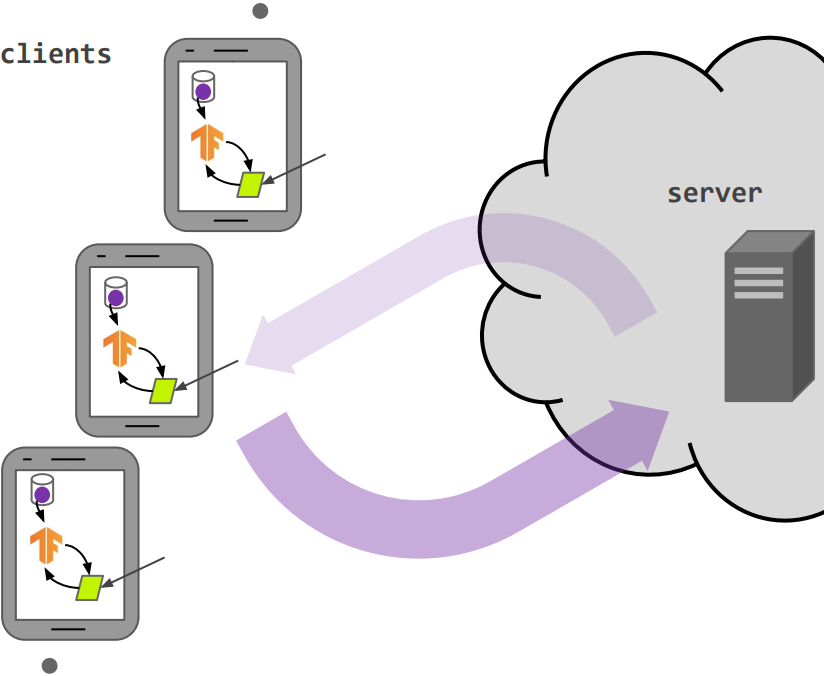
\includegraphics[width=0.7\textwidth]{Images/diagrams/FL_simplified.png}
        \decoRule
        \caption[FL system, simplified topology]{Simplified topology of an FL system \cite{survey_B}: \href{https://arxiv.org/abs/1912.04977}{URL}.}
        \label{fig: FL simplified topology}
\end{figure}

\section{Motivation}
Most FL research, to our knowledge, focuses on simulations and treats edge devices as black boxes; generally ignoring their nature and constrains. Taking in consideration the complexities of implementing ML on hardware, recent advancements in FL might be diminished or invalidated. The main motivation of this thesis is to identify, explore and possibly overcome the intrinsic conflicts that exist between FL and Artificial Neural Network (ANN) training in Field Programmable Gate Arrays (FPGA)s. % Such conflicts can be the batch size, where in FL tends to be minimized.

Instead of being incompatible, these two technologies may complement each other, which is worth investigating. Frequently in FL, transformations are applied on the generated ANN variables to reduce network utilization and enhance privacy. These transformations, which include quantization \cite{Mills2020}, adding Gaussian noise \cite{Wei2020} and others, tend to be spatially independent and could be implemented highly efficiently in hardware accelerators like FPGAs.

Finally, FL literature is almost devoid of wall-clock time examples. This thesis aims to provide a real world FL implementation that may be considered as a benchmark for future research. Furthermore, in order to be extendable and utilized in future works, the FL implementation is modular and platform independent.

\section{Scientific Contributions}
% The main focus of this thesis is combining FL training with FPGA based ANN implementations, while exploring and overcoming their inherent conflicts. Furthermore, it focus on the mostly unexplored FL setting of small client pools and its implicit difficulties. Finally, it provides a real world implementation of FL that can be used as a benchmark for future works. This FL implementation is agnostic of the ANN training implementation and can be used as a starting point for future works.
The main aim of this thesis is to explore the feasibility and efficiency of FL systems that employ FPGAs for the underlying training, focused on the edge setting. To achieve this, such a system was developed, thoroughly tested and benchmarked. Its components that can be utilized as starting points, examples or benchmarks of future works are as follows:
\begin{itemize}
    \item An FL system that is agnostic of the underlying ML model and training method. In the context of this work, it is employed with multiple ANNs of various types that are trained on CPU, GPU and FPGA. It can be easily modified to encompass other models and training implementations.
    \item A robustness analysis which focuses on the mostly unexplored FL setting of small client pools and its inherent difficulties.
    \item An FPGA-based implementation of training a CNN, that is optimized for the parameter space where the FL process is most efficient.
    \item Wall-clock timings of the CNN implementation and overall FL system, compared with equivalent implementations based on other technologies.
\end{itemize}
Finally, the aforementioned analyses and benchmarks are analyzed to provide apt suggestions for future works.

\section{Thesis Approach}
As the thesis moves forward, conflicts in terms of design and implementation are anticipated to arise between the two technologies. Furthermore, this is an mostly unexplored field. As such, a conservative and steady approach is expected to work best. 

Initially, a FL implementation that is agnostic and independent of the underlying training implementation, is developed. Its robustness is thoroughly validated, using TensorFlow to facilitate the local training. Subsequently, an FPGA-based CNN training implementation is created. 

Furthermore, an intermediate layer that connects the networking code of the FL clients with the FPGA driver is developed. With this approach, the FL implementation is combined with the FPGA-based implementation, and the overall system can be thoroughly tested and validated.

Finally, to benchmark the system, CPU and GPU implementation are developed and compared with it.

\section{Thesis Outline}
\begin{itemize}
    \item \textbf{Chapter 2 - Theoretical Background:} Description of the theoretical background of ML and FL.
    \item \textbf{Chapter 3 - Related Work:} Related works on FL, optimization techniques and hardware implementations of it.
    \item \textbf{Chapter 4 - FL architecture \& design:} Description of the FL architecture, design and implementation developed.
    \item \textbf{Chapter 5 - Robustness Analysis:} Analysis of the quality and performance of the FL implementation.
    \item \textbf{Chapter 6 - FPGA Implementation:} Description of the ANN architecture, design and implementation on FPGA developed.
    \item \textbf{Chapter 7 - Results:} Analysis of the quality and performance of the complete system. Comparisons with other technologies.
    \item \textbf{Chapter 8 - Conclusions and Related Work:} Conclusions and proposals for related future works.
\end{itemize}
\chapter{Theoretical Background}
\label{Chapter-Theoretical-Background}

%%%%%%%%%%%%%%%%%%%%%%%%%%%%%%%%%%%%%%%%%%%%%%%%%%%%%%%%%% Artificial Intelligence & Machine Learning %%%%%%%%%%%%%%%%%%%%%%%%%%%%%%%%%%%%%%%%%%%%%%%%%%%%%%%%%%
\section{Artificial Intelligence \& Machine Learning}
Various researchers and textbooks may provide different definitions of Artificial Intelligence (AI). Depending the school of though, AI is an artificial actor that thinks or acts, rationally or human-like, depending on what it knows. Generally, AI can be described as the study of intelligence agents. It is a modern science that encompasses a large variety of sub-fields, ranging from general-purpose areas, such as learning, to specific tasks like playing chess and giving medical diagnoses. AI can be relevant to any intellectual field, as it systematizes and automates intellectual tasks. \cite{russell_norvig_2003_1}

Machine learning (ML) is an AI field in which agents, in addition to the performance element, include a learning element that utilises their past experiences to enhance their behaviour. The core idea behind ML is that perception should be used to improve the ability to act in the future, not simply react in the present. Designing a learning element is a multi-facet problem that is affected by three major issues. \cite{russell_norvig_2003_18}

\subsection{Information management}%TODO:find a better title
The first issue is determining what information what information is useful and how it should be utilized. Different components of the input and output data should be learnt depending on the context in which the learning actor operates. One method is to directly link the current state of the actor or the world to their actions. Sometimes it can be more appropriate to infer relevant patterns from the data while ignoring unnecessary information. Another way is to collect action-value information indicating the desirability of actions based on their effect in the world state. These and other options may need to be combined in order to extract the most meaningful knowledge from the available data.

A common example is feature extraction. In ML, a feature \cite{Elgendy2020_ml_feature} is an individual measurable property or characteristic of a phenomenon being observed. They can be generic, such as edges in an image, or specialized, such as wheels and animal height. Feature extraction is the process of transforming such raw data into numerical features that can be processed.
\begin{figure}[H]
    \centering
        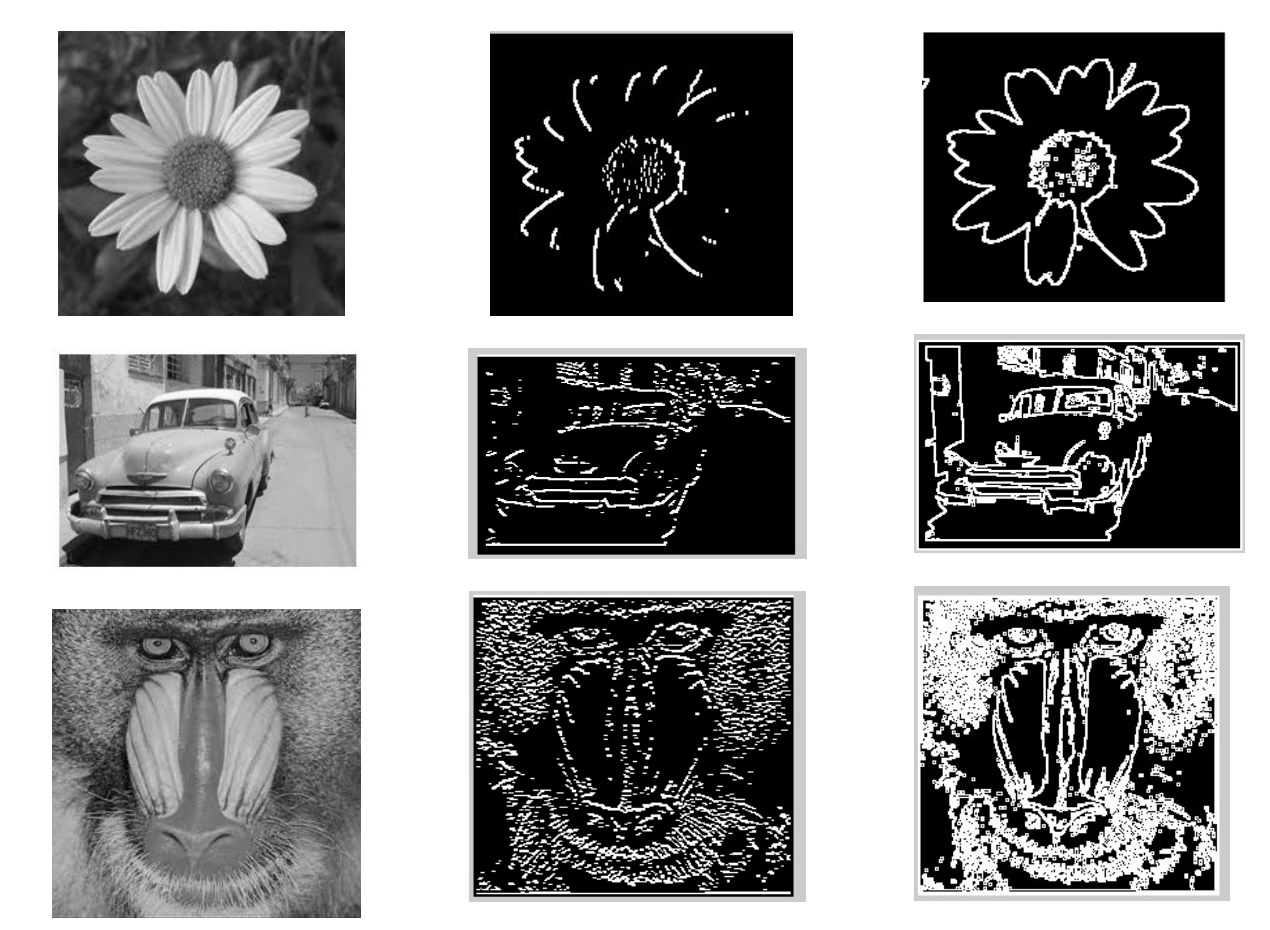
\includegraphics[width=0.8\textwidth]{Images/edge_detection.png}
        \decoRule
        \caption[Edge detection in greyscale images]{Edge detection in greyscale images: \href{https://aryamansharda.medium.com/how-image-edge-detection-works-b759baac01e2}{URL}.}
        \label{fig:Edge detection in greyscale images}
\end{figure}

Another key factor when designing learning systems is the availability of prior knowledge. Researchers have extensively looked into the issue where the agent uses only information that they encounter, but ways for transferring prior knowledge have been devised to speed up learning and improve decision-making.\cite{Transfer_Learning}

\subsection{Feedback mechanism}
The type of feedback available has a significant impact on the design and is perhaps the most crucial aspect of the learning problem. Usually three major types are distinguished: supervised, unsupervised, and reinforcement learning.

Supervised learning problems involve learning functions between sets of inputs and outputs. This is the case of a fully observable environments where the effects of the actors actions are immediately visible or the existence of a third party providing the correct solutions.

Unsupervised learning problems, on the other hand, do not supply output values and learning patterns are solely based on the input. As it has no knowledge of what constitutes a correct action or a desired state, an unsupervised learning agent cannot learn what to do. The hope is that through mimicry, the algorithm will generate imaginative content from it. This is a common scenario for probabilistic reasoning systems or when generating output data is prohibitively expensive. For the last case, a semi-supervised learning setting, in which only a subset of the outputs is generated, might be useful.

In the reinforcement learning setting there is no correct output provided, instead a reward is given to actor appropriate to the desirability of their actions. This is common when the world which the actor take part in continuously change according to their actions, or a desirable or undesirable state may be reached after a series of actions.

\subsection{Representation of the learned information}
The representation of the learned information is another important factor in establishing how the learning algorithm should operate. Common schemes include linear weighted polynomials for utility functions, propositional or first order logic, probabilistic representations like Bayesian Networks\cite{Probabilistic_Reasoning} and ANNs\cite{McCulloch1943}, and other methods have all been created.

%%%%%%%%%%%%%%%%%%%%%%%%%%%%%%%%%%%%%%%%%%%%%%%%%%%%%%%%%%%%%%%%%%%%%%%% Deep learning %%%%%%%%%%%%%%%%%%%%%%%%%%%%%%%%%%%%%%%%%%%%%%%%%%%%%%%%%%%%%%%%%%%%%%%%%
\section{Deep learning}
Deep learning is a sub-field of ML, partially overlapping with big data science. It consists of algorithms that use the perceptron as their basic building block, which is a mathematical function based on the McCulloch-Pitts model of biological neurons. They typically have hundreds of thousands to millions of perceptors with a variety of designs and topologies. Deep learning architectures include Deep Neural Networks (DNN)s, Convolutional Neural Networks (CNN)s, Recurrent Neural Networks (RNN)s and others, each one offering different capabilities and options.
\begin{figure}[H]
    \centering
        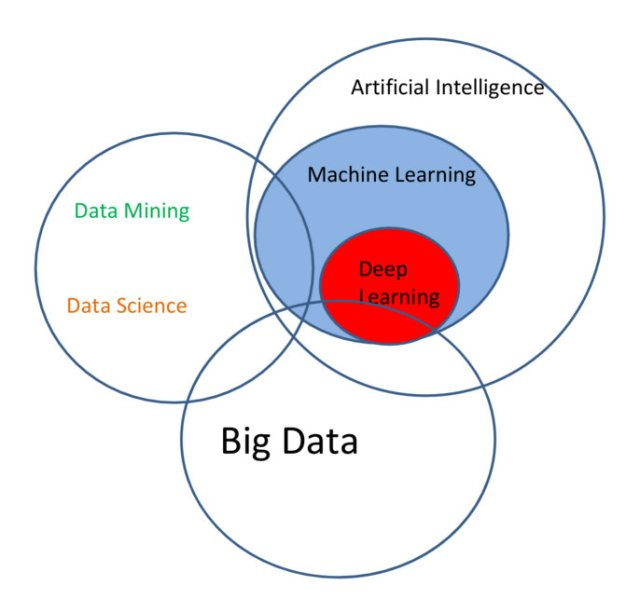
\includegraphics[width=0.6\textwidth]{Images/diagrams/ai_data_science.jpg}
        \decoRule
        \caption[AI Venn Diagram]{AI, ML, DL, Data Mining, Data Science, and Big Data: \href{https://whatsthebigdata.com/2016/10/17/visually-linking-ai-machine-learning-deep-learning-big-data-and-data-science/}{URL}.}
        \label{fig:AI Venn Diagram}
\end{figure}

Deep learning applications have demonstrated human-like or superior capabilities in several scientific and commercial fields such as image\cite{Alexnet} and speech\cite{limits_speech_recognition} recognition, natural language processing\cite{natural_language}, climatology\cite{Climatology} and biotechnology\cite{biotechnology}. Due to these exceptional capabilities and wide range of applications, deep learning has attracted a large number of researchers from various scientific domains, resulting in its tremendous expansion. However, the science is still young and there are a number of challenges to be overcome. Expecting deep learning combined with improved data processing being a solution to computers gaining generic human-like intelligence (human equivalent AI) is still a distant dream.\cite{dl_evolution}

Historically, the field of deep learning emerged in 1943 with the inception of the aforementioned McCulloch-Pitts perceptron. In 1949, Donald Hebb noted out in his book "The Organization of Behavior" that neural pathways are strengthened each time they are utilized, a principle that is crucial to how humans learn. He claimed that when two nerves fire at the same moment, the link between them is strengthened. This progress resulted in the creation of the first real-world application of ANNs, "MADALINE" an adaptive filter that eliminates echoes on phone lines. In 1962, Widrow \& Hoff developed a learning procedure that distributed the error across the ANN, resulting in its eventual elimination. Despite these advances, deep learning research plummeted due to a variety of internal and external factor, including the widespread use of fundamentally faulty learning function and the adoption of von Neumann architecture across computer science.

\begin{figure}[H]
    \centering
        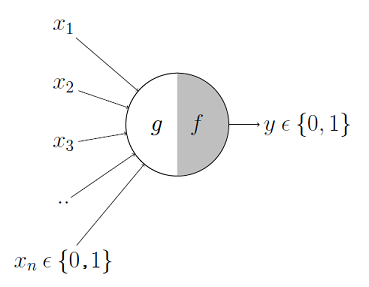
\includegraphics[width=0.6\textwidth]{Images/ANNArchitectures/McCulloch-Pitts Neuron.png}
        \decoRule
        \caption[McCulloch-Pitts Neuron]{The McCulloch-Pitts Neuron: \href{https://towardsdatascience.com/mcculloch-pitts-model-5fdf65ac5dd1}{URL}.}
        \label{fig:McCulloch-Pitts Neuron}
\end{figure}

Deep learning research stagnated until 1975, when developments such as Werbos' backpropagation and the building of the first multilayered network reignited interest in the field. Since then, the field continues to expand with innovations like hybrid models and ANN pooling layers. The current focus is on developing deep learning-specific hardware, as fast and efficient ANNs rely on it being defined for their use. Generally, architectures based on accelerators such as GPUs and FPGAs, or VLSI hardware-based designs, outperform CPU-based architectures. \cite{dl_history}

\subsection{Artificial Neuron}
As previously stated, the perceptron, also known as the artificial neuron, is the fundamental building element of the deep learning algorithms. In its simplest form, the artificial neuron receives one a set of inputs and sums it to produce an output. In practice, each input is weighted, then summed with a bias variable that acts as a threshold value, and the output is produced using an activation function.

The mathematical formula of the artificial neuron is defined as:
\begin{equation}
	y = \Phi( b + \sum_{i=1}^{I}x_i*w_i )
	\label{eqn:Artificial Neuron}
\end{equation}
Where:
\begin{conditions}
    y & output\\
    b & bias\\
    I & number of inputs \\
    \Phi & activation function\\
    w & weight
\end{conditions}

\subsection[Activation Functions]{Activation Functions \footnote{Also called transfer functions.}}
The activation function\cite{activation_function} of the artificial neuron is arguably its most important feature. It specifies how the weighted total of the inputs is transformed into an output (a target variable, class label, or score). Sometimes they limit their output range and are called squashing functions. There are various functions that are used as activation functions, with different properties and use cases each.

Most activation function are usually nonlinear so that the output varies nonlinearly with the inputs. With a linear activation function, regardless of how many layers a ANN has, it would behave just like a single-layer perceptron, as stacking linear functions creates just another linear function. Nonlinearity is, arguably, the most important aspect of the activation functions.

Activation functions are usually differentiable, which means that for a given input value, the first-order derivative can be determined. This is necessary because ANNs are mostly trained using the backpropagation of error algorithm, which requires the derivative of prediction error to update the model's parameters.

\subsubsection{Binary Step}
This is arguably the most basic activation function, as it was originally used in the McCulloch-Pitts Neuron and operates like a simple threshold. It activates the output of the perceptron when a certain value is exceeded, else the output is set as zero.
\begin{equation}
	f \left( x \right) = \left\{
    	\begin{array}{ll}
    	    0 & x \leq threshold\\
    	    1 & x > threshold\\
    	\end{array} 
	\right.
	\label{eqn:Binary step}
\end{equation}

\subsubsection{Sigmoid}
Also known as the logistic function, it normalizes and squashes the output of the neuron between 0 and 1. Its most important properties are that the output is barely affected by extreme values and the derivative is easily calculated.
\begin{equation}
	f \left( x \right) = \frac{1}{1+e^{-x}}
	\label{eqn:Sigmoid}
\end{equation}

\subsubsection{ReLU}
Because of its simple implementation, non-linearity, and high performance, the Recti-Linear Unit or ReLU function is arguably the most commonly utilized function in ANNs. It combines the binary step function for negative values and the identity function for positive values.
\begin{equation}
	f \left( x \right) = \left\{
    	\begin{array}{ll}
    	    0 & x \leq 0\\
    	    x & x > 0\\
    	\end{array} 
	\right.
	\label{eqn:ReLU}
\end{equation}

\subsubsection{Softmax}
Softmax ensures that all the outputs sums to 1 by normalizing them to a probability distribution. As such, it is mostly used as the final activation function in multi-decision ANN models.
\begin{equation}
	f \left( x \right)_{i} = \frac{e^{x_i}}{\sum_{k=1}^{K}e^{x_{j}}}
	\label{eqn:Softmax}
\end{equation}

\subsection{Artificial Neural Network architectures}
ANNs are collections of artificial neurons, typically organized in layers. Different layers may utilize different activation functions and/or apply different transformations to their inputs. Generally, the outputs of one layer's neurons are connected with the inputs of the following layer's neurons. If this holds true for all neurons in the ANN, the ANN is "fully connected". Alternatively, connections can be sparser, or loops between one or more layers can be created, giving the ANN different traits and capabilities.

When designing a layer, its position in the ANN is probably one of the most important variables. The input layer is the layer that accepts external data and is significantly dependent on the structure of the input; text input requires quite different management than visual input. The output layer is the layer that generates the final result, and its primary design factor is the nature of the output, which can be a yes or no answer, a classification or a set of probabilities. Usually, in order to have a human-readable output, specialized activation functions like softmax are used.

\subsubsection{Deep Neural Network (DNN)}
Between the input and output layers, there can be zero or more "hidden" layers. Typically, the majority of the network's computation takes place in these layers, and their design is influenced by a variety of criteria such as the nature of the problem and the input, available processing resources, and the required minimum capabilities. A DNN is defined as a ANN that has multiple hidden layers.\cite{IBM_Neural_Networks}
\begin{figure}[H]
    \centering
        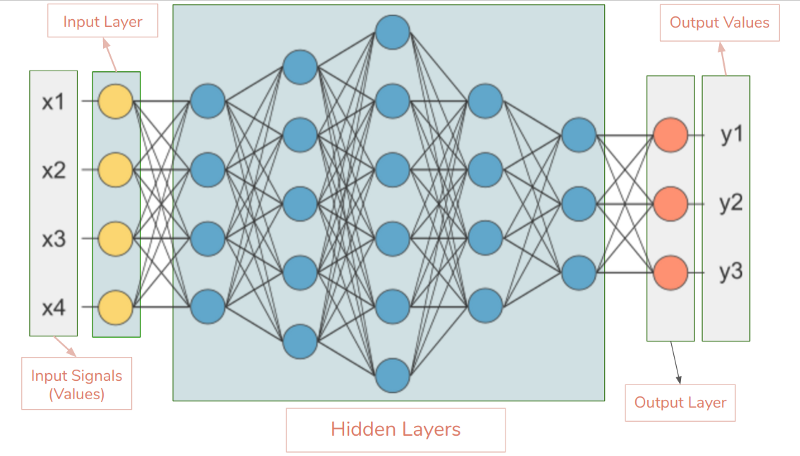
\includegraphics[width=0.8\textwidth]{Images/ANNArchitectures/dnn.png}
        \decoRule
        \caption[Deep neural network]{DNN with 5 hidden layers: \href{http://www.gabormelli.com/RKB/Multi_Hidden-Layer_(Deep)_Neural_Network}{URL}.}
        \label{fig:Deep neural network}
\end{figure}

\subsubsection{Convolutional Neural Network (CNN)}
The introduction of CNNs\cite{CS231n_stanford_cnn} is arguably one of the most significant achievements in the field of Deep Learning. They excibit great performance in image and video recognition, recommender systems, image classification, image segmentation, medical image analysis, natural language processing, brain-computer interfaces, and computer vision, among other applications. They perform best when the input is an image or a succession of images, but they are also effective in other scenarios.

CNNs are distinguished by their use of convolutional and subsampling layers, which enable the creation of multiple filters that can be trained in parallel. These filters are utilized to isolate and extract features from input data that would be undetectable by simpler DNNs. Subsequently, in order to get a result, the output of these filters is fed to fully connected layers. The design and depth of these filters are directly responsible for the network's feature extraction capabilities.

\begin{figure}[H]
    \centering
        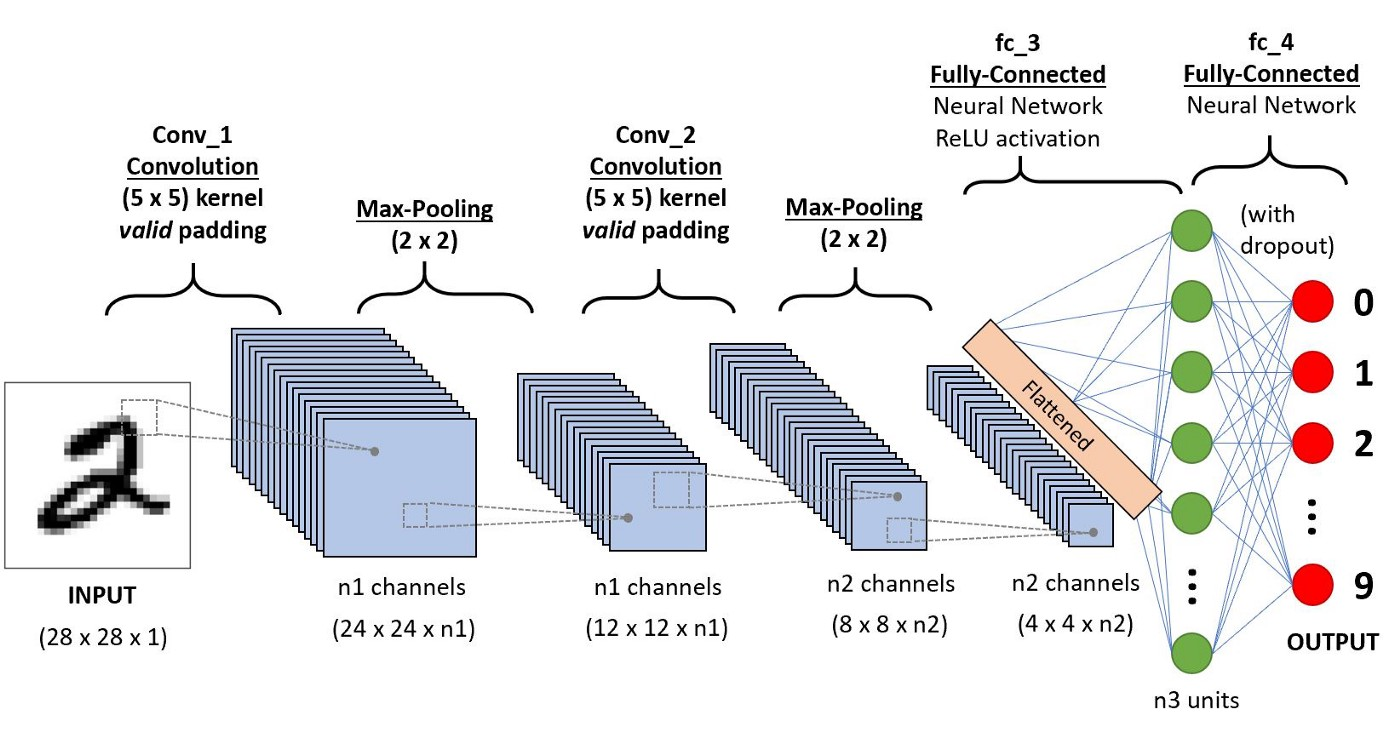
\includegraphics[width=1\textwidth]{Images/ANNArchitectures/cnn_2conv_layers.jpg}
        \decoRule
        \caption[A CNN sequence to classify handwritten digits]{A CNN sequence that classifies handwritten digits using 2 convolutional layers: \href{https://towardsdatascience.com/a-comprehensive-guide-to-convolutional-neural-networks-the-eli5-way-3bd2b1164a53}{URL}.}
        \label{fig:A CNN sequence to classify handwritten digits}
\end{figure}

Convolutional layers carry out the convolution process with the help of small matrices known as kernels. The kernel is the beating heart of a layer, and its type and dimensionality determine how the layer functions. Typically, two-dimensional kernels are used, while their size is mainly depended on the size of the input and their position on the network. A single convolutional layer can usually only produce filters that detect generic low-level features, such as edges and color. In order to create more specialized filters that can detect high-level features, multiple layers are used.

\begin{figure}[H]
    \centering
        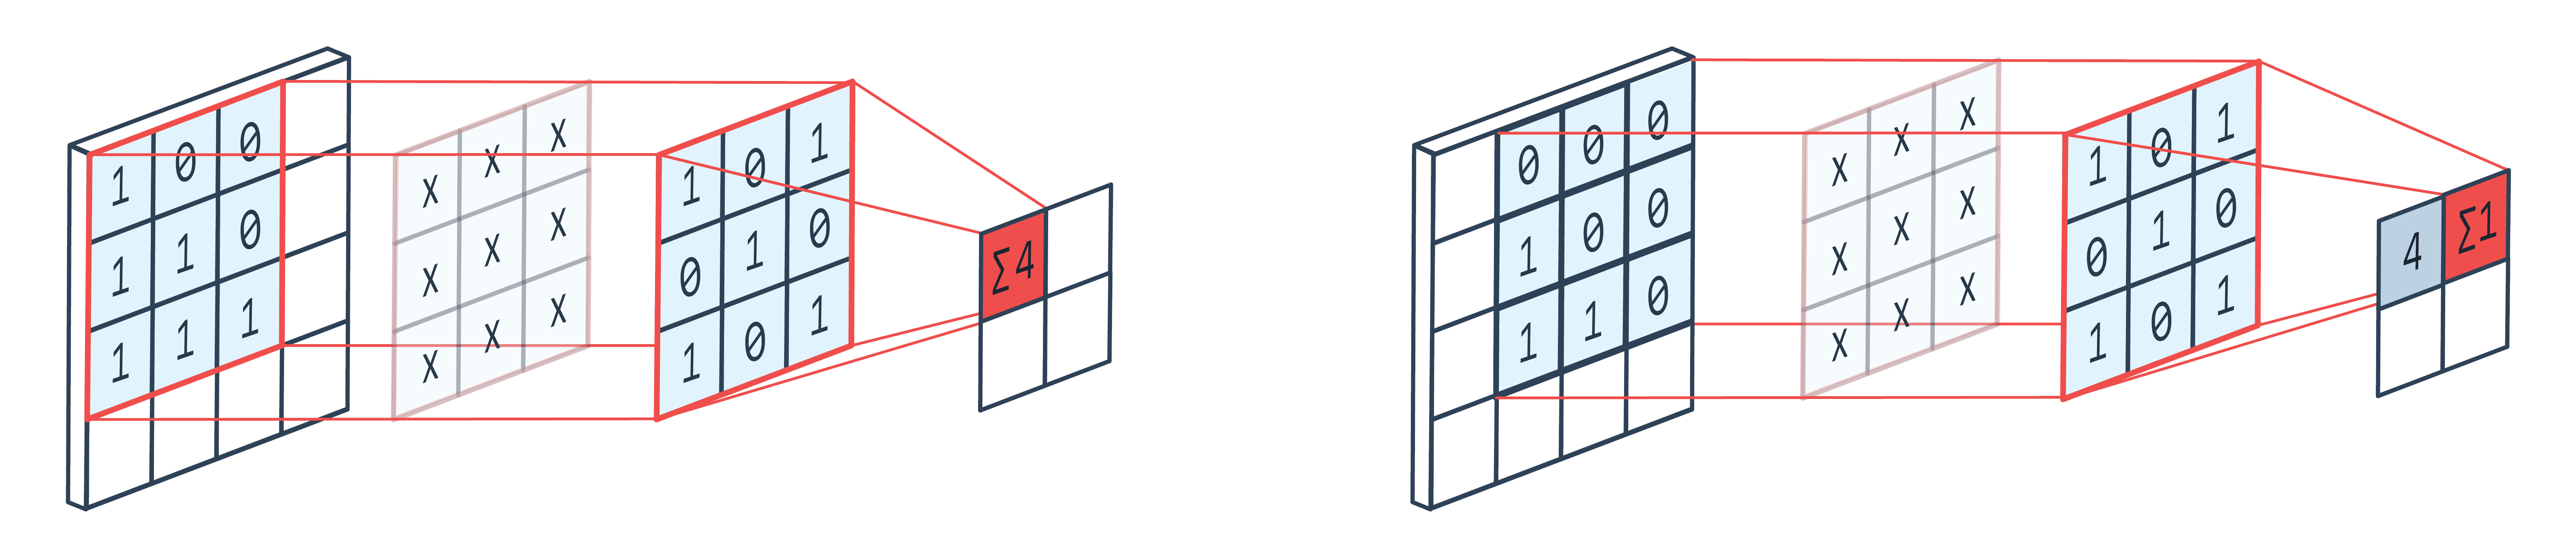
\includegraphics[width=1\textwidth]{Images/ANNArchitectures/2d_convolution.png}
        \decoRule
        \caption[2D convolution]{2D convolution: \href{https://peltarion.com/knowledge-center/documentation/modeling-view/build-an-ai-model/blocks/2d-convolution}{URL}.}
        \label{fig:2D convolution}
\end{figure}

The subsampling layers is the second distinguishing innovation of CNNs. Their primary task is to enable the network to recognize features without relying on their exact location. Furthermore, they simplify the network by reducing its number of parameters. Typically, they immediately follow convolutional layers in order to decrease the size of the features. Common subsambling layers include max pooling, mean pooling and others.

\begin{figure}[H]
    \centering
        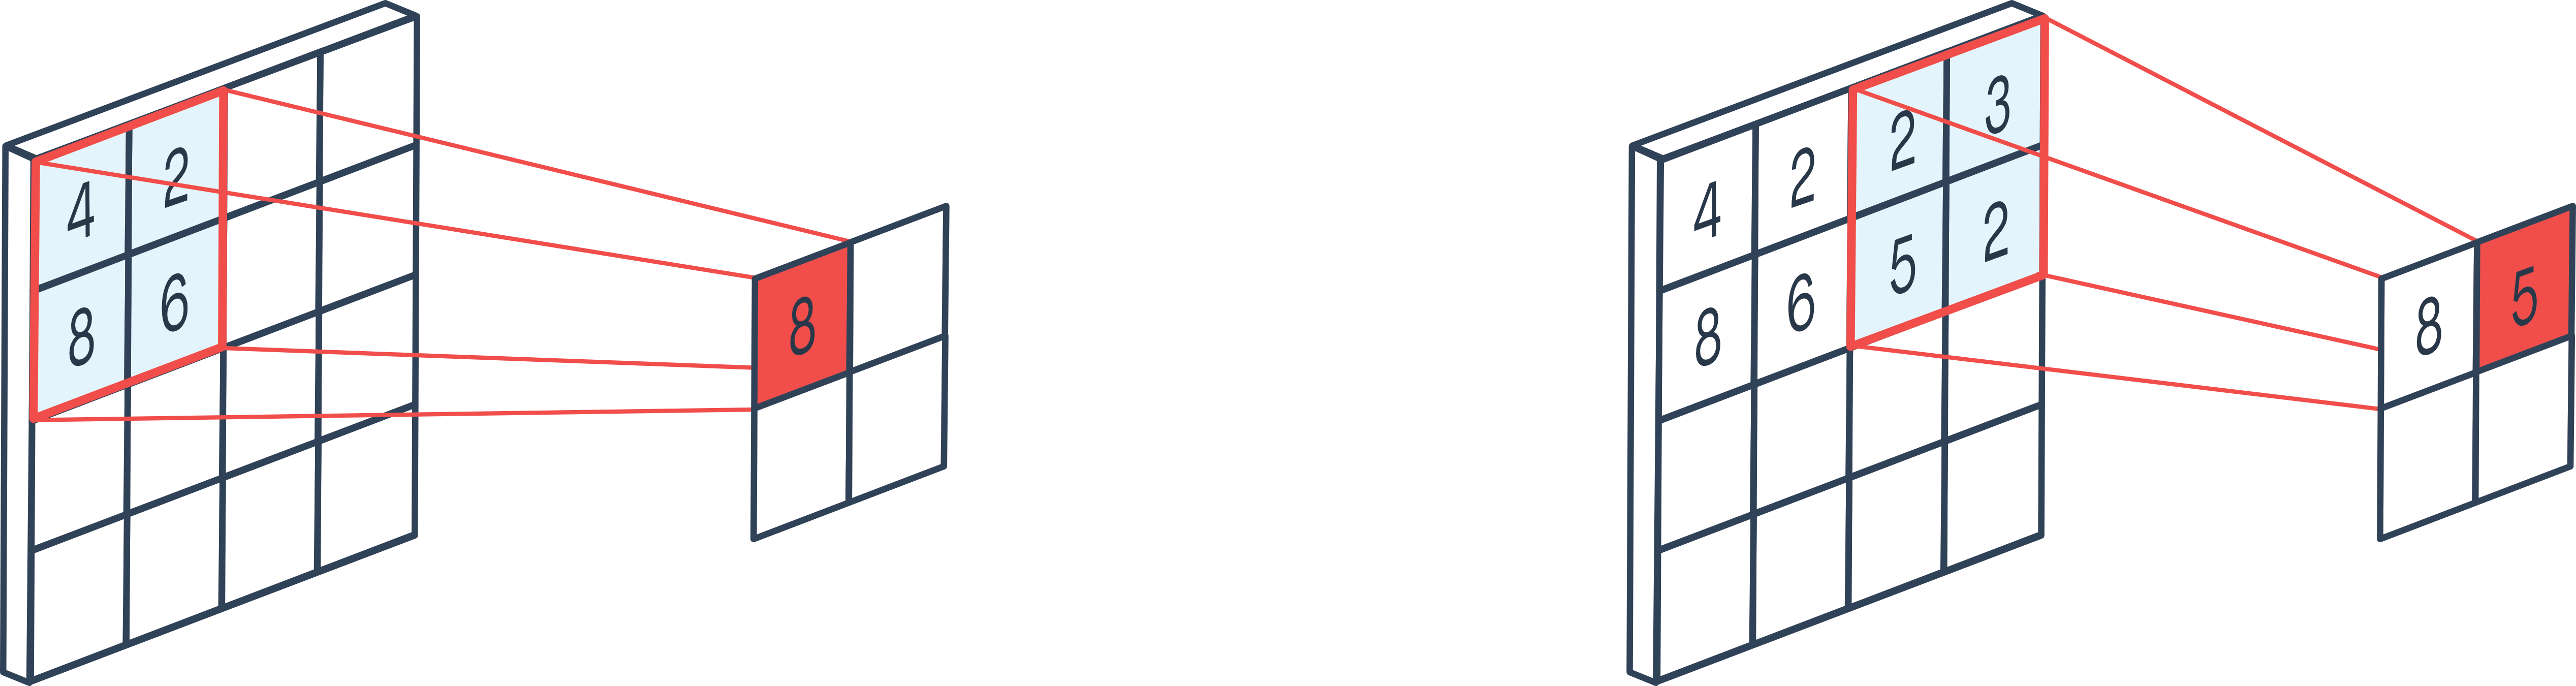
\includegraphics[width=0.76\textwidth]{Images/ANNArchitectures/2d_max_pooling.png}
        \decoRule
        \caption[2D max pooling]{2D max pooling: \href{https://peltarion.com/knowledge-center/documentation/modeling-view/build-an-ai-model/blocks/max-pooling-2d}{URL}.}
        \label{fig:2D max pooling}
\end{figure}

% \subsubsection{rnn?}

\section{Training Artificial Neural Networks}
As previously stated, ANNs are made up of neurons, which contain multiple parameters known as weights and biases, which are generally referred simply as weights. Training\footnote{Also called fitting.} is an iterative process that aims to improve the ANN's performance by optimizing these parameters. To accomplish this, three key elements are required: a loss function, an optimization algorithm such as gradient descent and a training algorithm like backpropagation.

In supervised learning, input-output examples are fed to the ANN. It produces predictions based on the inputs and then uses the loss function to compare these predictions to the intended outputs. The loss function calculates the ANN's error, which is a quantifiable difference between the expected and actual output. The error gradients of the ANN's weights are then determined, commonly using the backpropagation process. Finally, the optimization algorithm uses the error gradients to generate new values for the weights that should perform better.

In unsupervised learning, only input examples are given. The ANN attempts to mimic the data it is given and optimizes itself using the mistake in its output. Instead of a loss function, the error is represented as the likelihood of an incorrect output. The error gradients can be computed using a variety of learning algorithms, such as Maximum Likelihood, Maximum A Posteriori, and others, rather than the predominantly used backpropagation in supervised learning. Finally, to generate new values for the ANN's weights, any optimization algorithm may be employed.

In reinforcement learning, the ANN produces a prediction and subsequently receives a feedback\footnote{Feedback is frequently given after a series of predictions.}, usually numerical, regarding its performance. The loss function uses this feedback and prediction, and like in the supervised learning, the error gradients are calculated through backpropagation. Finally, the ANN's weights are updated using a optimization algorithm.

The training technique varies greatly depending on the problem, the ANN architecture, and numerous other factors, but it is always iterative. An epoch is typically defined as using all of the data points in the training set once.

\subsection{Initialization}
The initialization of the ANN's weights has a significant impact on the ANN's final performance and training time. Naive methods, such as zeroing all weights or assigning them fully random values, might produce detrimental effects. If the weights in a ANN start out too small, the signal will shrink as it passes through each layer, eventually becoming too small to be useful. Likewise, if the weights in an ANN start out too large, the signal grows too huge as it goes through the layers, eventually overwhelming all other signals. As a result, the ANN may require a significant amount of training time or possibly become stuck in its initial state and not converge to a solution.

One common ANN initialization scheme used to solve this problem is called Glorot\footnote{also known as Xavier. \cite{Xavier_initialization}} Initialization\cite{pmlr-v9-glorot10a, Glorot_initialization_large}. The idea is to initialize each variable with a small Gaussian value with mean of 0 and variance based on its fan-in and fan-out\footnote{In a fully connected ANN, the fan-out of a layer equals the fan-in of the next layer.}. The Glorot Initialization not only outperforms uniform random initialization (in most circumstances), but it also eliminates the need to determine appropriate fixed limit values. There are actually two versions of Glorot initialization, Glorot uniform and Glorot normal, with different distribution and variance.

The variance of the Glorot Initialization is defined as:

\noindent\begin{minipage}{.5\linewidth}
    \begin{equation}
    	V \left[ W_i \right] = \frac{2}{n_i+n_{i+1}}
    	\label{eqn:Glorot Initialization variance, uniform distribution}
    \end{equation}%
    \captionof*{figure}{Uniform distribution}
\end{minipage}%
\noindent\begin{minipage}{.5\linewidth}
    \begin{equation}
    	V \left[ W_i \right] = \frac{\sqrt{6}}{\sqrt{n_i + n_{i+1}}}
    	\label{eqn:Glorot Initialization variance, normal distribution}
    \end{equation}
    \captionof*{figure}{Normal distribution}
\end{minipage}
Where:
\begin{conditions}
    V & variance\\
    i & layer\\
    W & weights\\
    n & fan-in of a layer\\
\end{conditions}

The Glorot initialization makes the assumption that the activations immediately after initialization are linear, as the initialized values are close to zero and their gradients close to 1. While this holds true for the traditional activation function its development was based on\footnote{Sigmoid, tanh and softsign.}, it is invalid for the more modern rectifying nonlinearities\footnote{ReLU and PReLU.} in which the non-linearity is at zero. As such, the He Initialization \cite{He_Init_paper, Glorot_He_initialization} was proposed, with Gaussian distribution and the following variance:
\begin{equation}
	V \left[ W_i \right] = \frac{2}{n_i}
	\label{eqn:He Initialization variance}
\end{equation}


\subsection[Loss Functions]{Loss Functions \footnote{Also called cost or error functions.}}
A loss function\cite{loss_functions} provides a real number that represents the error a function associated with an event. In Deep Learning, it quantifies the inaccuracy of a ANN. The training algorithm tries to minimize this number by altering the ANN's weights, in hopes that it improves the network's accuracy. The choice of loss function is influenced by the nature of the input, as well as by the nature of the output. Some of the most common loss functions are listed below.

\subsubsection{Regression Loss Functions}
Regression problems involve predicting numerical values, a number or set of numbers. This is a usual problem in supervised learning. The appropriate loss functions measure the distance between the prediction and the ideal values.

The most frequent regression loss function is Mean Squared Error (MSE). This method is utilized when the prediction belong to a continuous plane. The MSE is the mean of the squared distances between the predicted values and the target variables.
\begin{equation}
    	Loss = \frac{ \sum_{i=1}^{n} \left( y_i^{target} - y_i^{pred.} \right)^2 } {n}
    	\label{eqn:Mean Squared Error}
\end{equation}

When the data are discrete values, the Poisson loss function is more appropriate. Under the assumption that the target comes from a Poisson distribution, minimizing the Poisson loss is equivalent of maximizing the likelihood of the data.
\begin{equation}
    	Loss = \frac{1}{N} \sum_{i=0}^{N} \left( y_i^{pred.} - y_i^{target}\log y_i^{pred.} \right)
    	\label{eqn:Poisson Error}
\end{equation}

\subsubsection{Classification Loss Functions}
In classification problems, the examples must be classified into one or more classes, which may or may not be preset. The ANN generates a probability distribution that represents its confidence in the example's classification.

Binary cross-entropy is a loss function that is used in binary classification tasks with predefined classes. These are tasks that answer a question with only two choices.
\begin{equation}
    	Loss = - 
    	\frac{1}{ \substack{ output\\ size } }
    	\sum_{i=1}^{ \substack{ output\\ size } }
    	y_i^{target} \cdot \log y_i^{pred.} + 
    	\left( 1 - y_i^{target} \right) \cdot
    	\log \left( 1 - y_i^{pred.} \right)
    	\label{eqn:Binary cross-entropy}
\end{equation}

In problems with more than one classes, the categorical cross-entropy loss function, a generalization of binary cross-entropy loss function, is most commonly used. The \( y_i^{target}\) is the probability that event \( i \) occurs and the sum of all these probabilities is 1, meaning that exactly one event may occur.
\begin{equation}
    	Loss = 
    	- \sum_{i=1}^{ \substack{ output\\ size } }
    	y_i^{target} \cdot \log y_i^{pred.}
    	\label{eqn:Categorical cross-entropy}
\end{equation}

Classification problems in unsupervised learning is quite different, as the desired output is not provided to the ANN. The most commonly used training algorithm is k-means clustering. It aims to partition the examples into a predefined number of clusters. To achieve this it tries to minimize the pairwise squared deviations of points in the same cluster. The equivalent to a loss function is defined as:
\begin{equation}
	\argmin_S \sum_{i=1}{k} \frac{1}{ \left| S_i \right| } \sum_{}{x,y \in S_i} \left\| x-y \right\|^2
	\label{eqn:k-means error}
\end{equation}
Where:
\begin{conditions}
    S & clusters\\
    x,y & points in cluster\\
\end{conditions}

\subsubsection{Reward Functions}
Reward functions serve the same goal as loss functions in that they quantify the accuracy of an ANN in order to optimize it, but in the opposite direction. Rather than penalizing the ANN, it rewards it based on its performance, with the learning algorithm aiming to maximize this reward. This is most frequently seen in Reinforcement Learning. Reward functions specify how the agent should behave, hence their structure is heavily influenced by the problem and the laws of the universe in which the agent lives. 

\subsection{Backpropagation}
Backpropagation\cite{backpropagation_original, Backpropagation_wiki} is a training algorithm for feedforward ANNs under supervised learning\footnote{Generalizations of the algorithm can be used for other network architectures and different training schemes.}. Feedforward ANNs refers to fully connected networks with no cyclical connections, most DNNs and CNNs adhere this standard. For a single example, backpropagation computes the gradient of the loss function with respect to the network weights. The gradient\cite{gradient_wiki} represent the direction and rate of fastest rise. If a function's gradient is non-zero at a point, the gradient's direction is the direction in which the function increases the fastest, and the magnitude of the gradient is the rate of growth in that direction, in respect of that point.

Backpropagation is sometimes misconstrued to mean the entire learning algorithm for ANNs. Backpropagation is merely the method for computing the gradient; another algorithm, such as stochastic gradient descent, is needed to accomplish learning using this gradient. Furthermore, backpropagation is frequently misinterpreted as being limited to ANNs while, in fact, it may compute derivatives of any function. Its use to ANNs is critical because it enables efficient training, especially when using hardware accelerators.

The ANN can be mathematically expressed as:
\begin{equation}
    g \left( x \right) \coloneqq f^L \left( W^L f^{L-1} \left( W^{L-1} \cdots f^1 \left(  W^1 x \right) \cdots \right) \right)
	\label{eqn:Feedforward ANN definition}
\end{equation}
Where:
\begin{conditions}
    x & input\\
    g(x) & prediction\\
    f^l & activation functions at layer \(l\)\\
    W^l & weights at layer \(l\)\\
    L & number of layers\\
\end{conditions}

Then the error function \(C\) with desired output \(y\) is:
\begin{equation}
    C \left( y , 
    f^L \left( W^L f^{L-1} \left( W^{L-1} \cdots 
    f^1 \left(  W^1 x \right) \cdots \right) \right) 
    \right)
	\label{eqn:Backpropagation, loss function}
\end{equation}

By using the chain rule the total derivative of the loss function is:
\begin{equation}
    \frac{\mathrm{d}C}{\mathrm{d}y} \circ 
    \left( f^L \right)' \cdot W^L 
    \circ \left( f^{L-1} \right)' \cdot W^{L-1} \cdots 
    \left( f^{1} \right)' \cdot W^{1}
	\label{eqn:Backpropagation, total derivative of the loss function}
\end{equation}

Given that the gradient \(\nabla \) in respect to the input is the transpose of the derivative in respect to the output, the total gradient can be determined as:
\begin{equation}
    \nabla_x C =
        \left( W^{1} \right)^T \cdot \left( f^{1} \right)' \cdots \circ
        \left( W^{L-1} \right)^T \cdot \left( f^{L-1} \right)' \circ
        \left( W^{L} \right)^T \cdot \left( f^{L} \right)' \circ
        \nabla_y C
	\label{eqn:Backpropagation, total gradient}
\end{equation}

The partial gradients at each layer\( \delta^l \), which represent the effect of the weights in the corresponding layers on the error function, may be easily determined by eliminating the effect of the previous ones:
\begin{equation}
    \begin{split} 
        \delta^{1} & = 
            \left( f^{1} \right)' \circ 
            \left( W^{2} \right)^T \cdot \left( f^{2} \right)' \cdots \circ
            \left( W^{L-1} \right)^T \cdot \left( f^{L-1} \right)' \circ
            \left( W^{L} \right)^T \cdot \left( f^{L} \right)' \circ
            \nabla_y C\\
        \delta^{2} & =
            \left( f^{2} \right)' \cdots \circ
            \left( W^{L-1} \right)^T \cdot \left( f^{L-1} \right)' \circ
            \left( W^{L} \right)^T \cdot \left( f^{L} \right)' \circ
            \nabla_y C\\
        \delta^{L-1} & =
            \left( f^{L-1} \right)' \circ
            \left( W^{L} \right)^T \cdot \left( f^{L} \right)' \circ
            \nabla_y C\\
        \delta^{L} & =
            \left( f^{L} \right)' \circ
            \nabla_y C\\
    \end{split}
	\label{eqn:Backpropagation, per layer gradient}
\end{equation}

A naive approach would be to compute these derivatives forward. Backpropagation, on the other hand, eliminates duplicate multiplications by employing dynamic programming, as the derivative of one layer can be used to calculate the derivative of the previous one. Furthermore, by going backwards, a vector \(\delta^l\) is multiplied by exactly one matrix \(\left( W^{l} \right)^T \circ \left( f^{L-1} \right)'\) at each step. When calculating forwards, however, each multiplication multiplies a matrix with \( L-l \) matrices, which is a far more expensive operation.

\subsection{Gradient Descent}
Gradient descent\cite{IBM_Gradient_Descent, gradient_descent_wiki} is an optimization algorithm which is commonly used to train ANNs. Gradients generated by training algorithms such as backpropagation are used to alter the network's weights, in order to produce the minimal possible error. Its basis is that a differentiable function \(F\) decreases fastest at a point \(a_n\), in the direction of the negative gradient of that point \(-\nabla F \left( a_n \right)\). Mathematically it is defined as:
\begin{equation}
a_{n+1} = a_n - \gamma \nabla F \left( a_n \right)
	\label{eqn:Gradient Descent}
\end{equation}

The learning rate parameter \(\gamma\) is the size of the step taken each time the algorithm is executed. It has a significant impact on the overall performance of the training procedure and should be fine-tuned. If it is too large, there is a high risk of overshooting the minimum of the function. If it is too small, more iterations are needed, and there is a risk too end up in a suboptimal local minimum.
\begin{figure}[H]
    \centering
        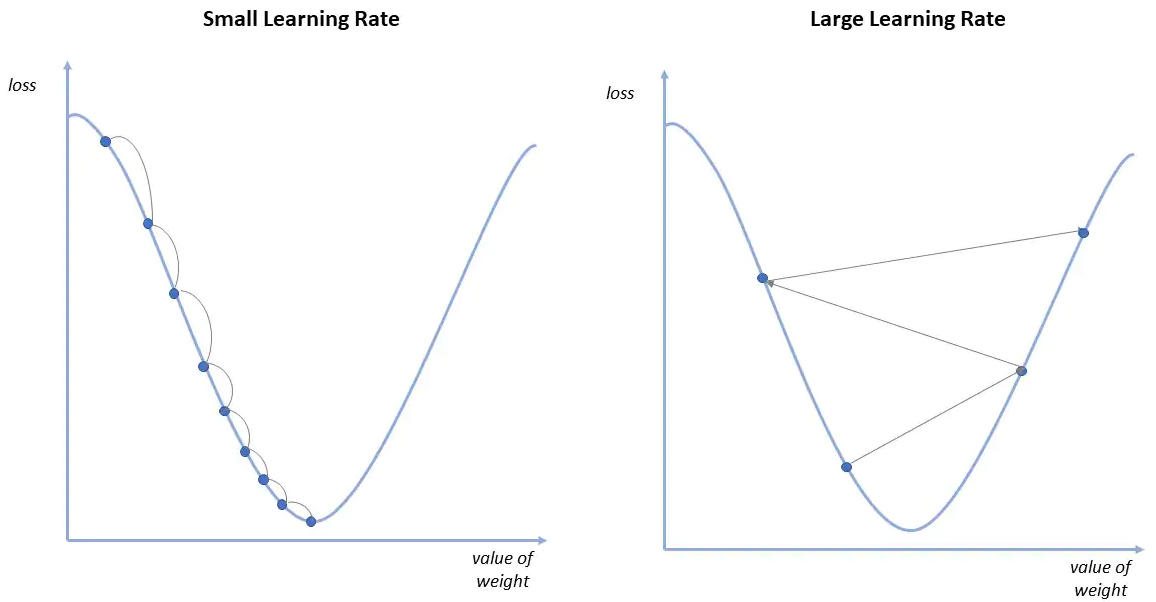
\includegraphics[width=0.8\textwidth]{Images/diagrams/learning_rate.png}
        \decoRule
        \caption[Effect of learning rate in Gradient Descent]{Effect of learning rate in Gradient Descent: \href{https://www.ibm.com/cloud/learn/gradient-descent}{URL}.}
        \label{fig:Learning rate in Gradient Descent}
\end{figure}

\subsubsection{Challenges}
Gradient descent faces challenges with local minima and saddle points, when the gradient gets close to zero the algorithm is unable to re-adjust the network's weights. Local minima resemble the global minimum in shape, trapping the algorithm. Saddle points are stable positions with no relative maximum or minimum, making it difficult for the algorithm to decide what to do.
\begin{figure}[H]
    \centering
        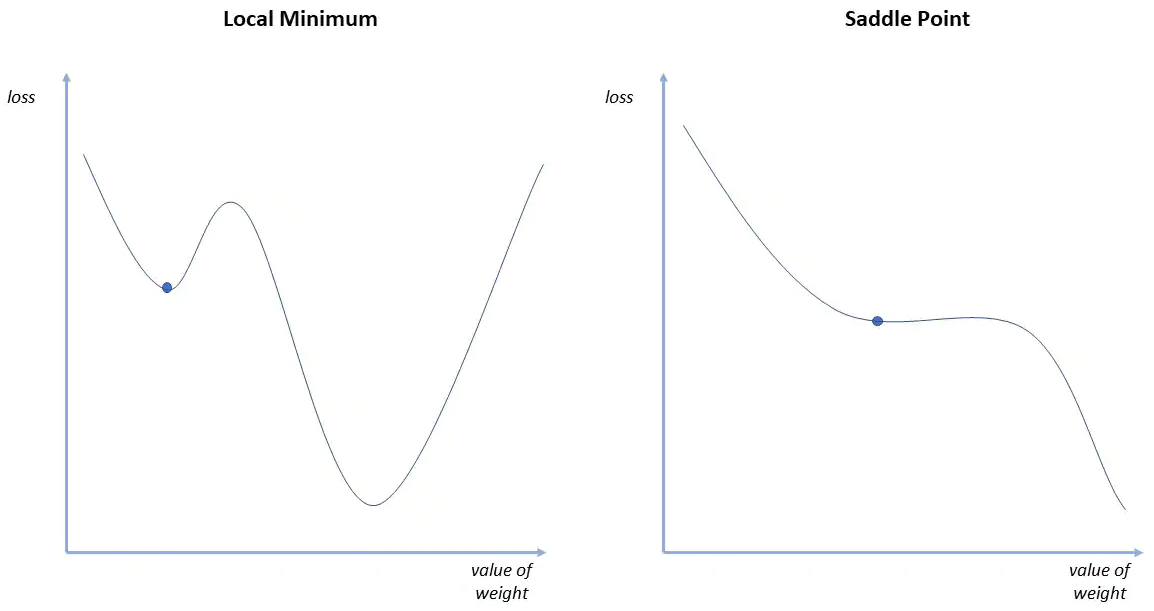
\includegraphics[width=0.8\textwidth]{Images/diagrams/LocalMinimum_SaddlePoints.png}
        \decoRule
        \caption[Local minimum and saddle point]{Local minimum and saddle point: \href{https://www.ibm.com/cloud/learn/gradient-descent}{URL}.}
        \label{fig:Local minimum and saddle point}
\end{figure}

To address this issue, a number of enhancements have been developed culminating in the Nesterov Momentum\cite{nesterov_momentum} extension. To accelerate the process, the first adjustment is to add a momentum variable, a percentage \(\beta\) of the previous iterations' change \(m\). Simply adding that tends to result in overshooting. To mitigate this, the calculation of the gradient takes the momentum of the previous steps into account. With Nesterov momentum, the gradient descent is defined as:
\begin{equation}
    \begin{gathered} 
        m_{n+1} = \beta m_n - \gamma \nabla F \left( a_n + \beta m_n \right)\\
        a_{n+1} = a_n + m_{n+1}\\
    \end{gathered}
	\label{eqn:Gradient Descent with Nesterov momentum}
\end{equation}

In deep ANNs with numerous or repeating hidden layers, training with backpropagation and gradient descend introduce the phenomenon of vanishing gradients. As the algorithm travels backwards through the layers, the gradients get smaller and smaller, eventually becoming insignificant and unable to alter the weights of the network. Non monotonic activation functions, such as ReLU, and more complex topologies, such as residual ANNs, are prevalent but not exclusive solution.

Another problem, especially frequent in RNNs, is exploding gradients. This occurs when a gradient gets too large, turning the model unstable. To address this, techniques such as dimensionality reduction have been developed, with the goal of reducing the model's overall complexity.

\subsubsection{Variations}
In vanilla Gradient Descent, each example's error is assessed, the gradients are produced and then the weights of the ANN are updated. In order to calculate the error of an example, the update of the prior one must be applied first. Since this process cannot be parallelized and must be repeated for each example, it is computationally inefficient.

Furthermore, the dataset is often used multiple times during the training of a model. In vanilla Gradient Descent, the examples are used in order. This pattern is often recognized by the models, which then introduce biases that lead to less-than-ideal solutions.

To address these inefficiencies, three key variations have been developed:

\begin{itemize}
    \item Batch Gradient Descent
\end{itemize}
Batch gradient descent performs backpropagation and updates the network only after calculating the loss function for \textit{all} the examples in the training dataset. The expensive operations of calculating the gradients and new weights occur just once per epoch, resulting in a computationally more efficient algorithm. Furthermore, the loss function can be parallelized indefinitely.

This method yields a stable error gradient and convergence, but it frequently leads to local minima. Furthermore, in order to calculate the loss, all of the data must be in memory, making the approach unsuitable for huge datasets. Finally, more passes through the dataset are needed, as updates are infrequent.

\begin{itemize}[resume]
    \item Stochastic Gradient Descent (SGD)
\end{itemize}
SGD works similarly to vanilla Gradient Descent, with the exception that the training examples are chosen at random. This eliminates the bias produced by consuming the examples in a particular order. Furthermore, its frequent updates produce noisy gradients, which aid in avoiding local minima.
    
\begin{itemize}[resume]
    \item Mini-batch Stochastic Gradient Descent
\end{itemize}
Mini-batch SGD builds on the ideas of the previous variations by splitting the training dataset randomly into small batches and performing updates on each one of them. This method achieves a balance between the computational efficiency of batch gradient descent and the randomness of SGD. This is by far the most popular variation, and it is commonly abbreviated just as SGD.

\subsection{Model Overfitting}
The goal of training ANNs is to improve their performance on real-world data, i.e. to generalize its knowledge. When training, the model\footnote{Most statistical models, not just ANNs, exhibit this phenomenon.} may sometimes fit exactly against training data, severely limiting its effectiveness with previously unseen data and negating its objective.

Training is typically conducted with a sample dataset. If the model trains on this for too long, or if the model is overly sophisticated, it may memorize irrelevant information, the "noise" within the training dataset. This is known as overfitting\cite{IBM_overfitting}, and the most common signs are unusually high accuracy on the training dataset and high variance within the predictions of the network.
\begin{figure}[H]
    \centering
        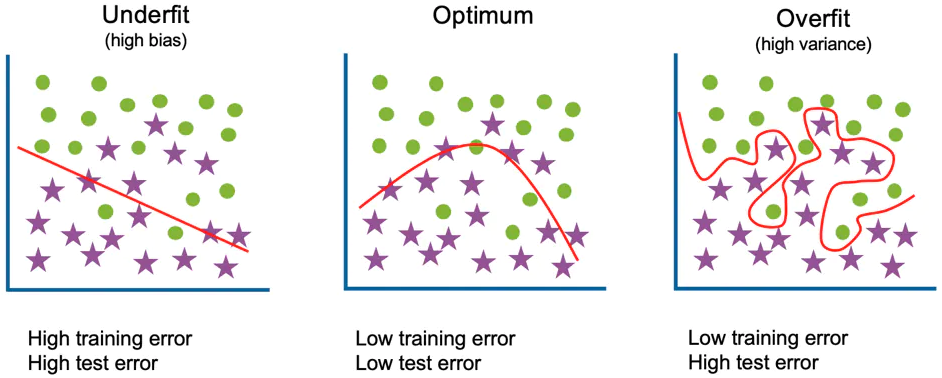
\includegraphics[width=1\textwidth]{Images/diagrams/model-over-fitting.png}
        \decoRule
        \caption[Model overfitting]{Model overfitting and its opposite, model underfitting: \href{https://www.ibm.com/cloud/learn/overfitting}{URL}.}
        \label{fig:Model overfitting}
\end{figure}

Multiple methods to avoid or suppress overfitting have been developed, some common ideas are listed below:
\begin{itemize}
    \item Early stopping
\end{itemize}
This method aims to stop the training before the model starts learning the noise within the model. To achieve this, a portion of the training dataset is held aside for testing rather than being used during training. This dataset is used to evaluate the ANN after each epoch, and if the accuracy is lower than before, training is terminated. There is a risk of stopping too soon and underfitting the model; a middle ground should be sought.
\begin{figure}[H]
    \centering
        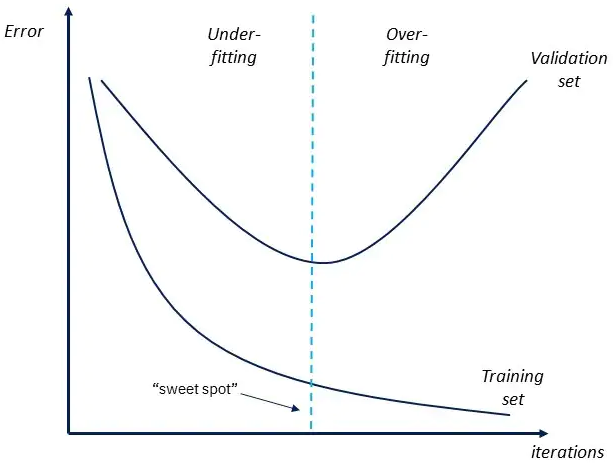
\includegraphics[width=0.6\textwidth]{Images/diagrams/classic_overfitting.png}
        \decoRule
        \caption[Overfitting/Underfitting]{Border between overfitting and underfitting: \href{https://www.ibm.com/cloud/learn/overfitting}{URL}.}
        \label{fig:Model Overfitting/Underfitting}
\end{figure}

\begin{itemize}[resume]
    \item Data manipulation
\end{itemize}
A common way to reduce overfitting is through manipulating the input data. Expanding the training dataset with real-world or machine-generated data can assist the model in identifying patterns between the input and output variables. When using clean and relevant data, this strategy is effective; otherwise, the model may grow too complex and overfit even more. Another technique is augmenting already existing data by adding noise to them. The goal is to help the model discern between useful and irrelevant patterns.

\begin{itemize}[resume]
    \item Model simplification
\end{itemize}
Multiple methods attempt to enhance the model's performance by simplifying it and the problem that is called to solve. Feature selection refers to a class of methods that enhance the training dataset by removing examples. Such methods include removing highly correlated features and incomplete examples, selecting the best features through statistical methods and others. Another family of methods, such as the Principle Component Analysis, seek to transform the features by reducing their dimension.

The preceding methods necessitate some level of domain knowledge, which is not always available. In this scenario, regularization methods are particularly helpful, as they aim to reduce complexity by altering the model. In general they try to penalize input parameters with large coefficients, typical in examples with significant noise, in order to minimize the variance in the model. Such methods include L1 regularization, dropout and others.

% \subsection{Adaptive Learning Rate?}
% \subsection{Adaptive algoritms?}
%%%%%%%%%%%%%%%%%%%%%%%%%%%%%%%%%%%%%%%%%%%%%%%%%%%%%%%%%%%%%%%%%%%%%% Federated learning %%%%%%%%%%%%%%%%%%%%%%%%%%%%%%%%%%%%%%%%%%%%%%%%%%%%%%%%%%%%%%%%%%%%%%
\section{Federated Learning}
%definition and central aim
Federated Learning \cite{FL-original-paper, FL_comprehensive_survey} (FL) is a ML setting in which multiple clients, ranging from big enterprises to personal mobile devices, collaborate to train a model under the supervision of a central server. The goal of this is to alleviate many of the systemic privacy problems associated with centralization by decentralizing the training data. Under FL, any model that employs SGD-like approaches can be trained. ANNs, linear regression, Support Vector Machines, and other models fall into this category. FL acts as a wrapper for ML; what is true for a model when trained locally tends to hold true when trained in a FL context.

% basic entities and operation
In general, the FL setting has two basic entities: data owners (participating clients) and model owners (orchestrating server). Participants never share their datasets, instead use them to locally train a model sent by the orchestrating server. The generated weights are shared, which the server aggregates them in order to construct a global model. The models trained by the clients are referred as local models whereas the aggregated model is referred as global model.

% basic topology
The entities are typically configured in a hub-and-spoke topology, as shown in figure \ref{fig:FL topology}, with the hub representing the coordinating server and the spokes connecting to the clients. The server organizes the training but never access the training data.
\begin{figure}[H]
    \centering
        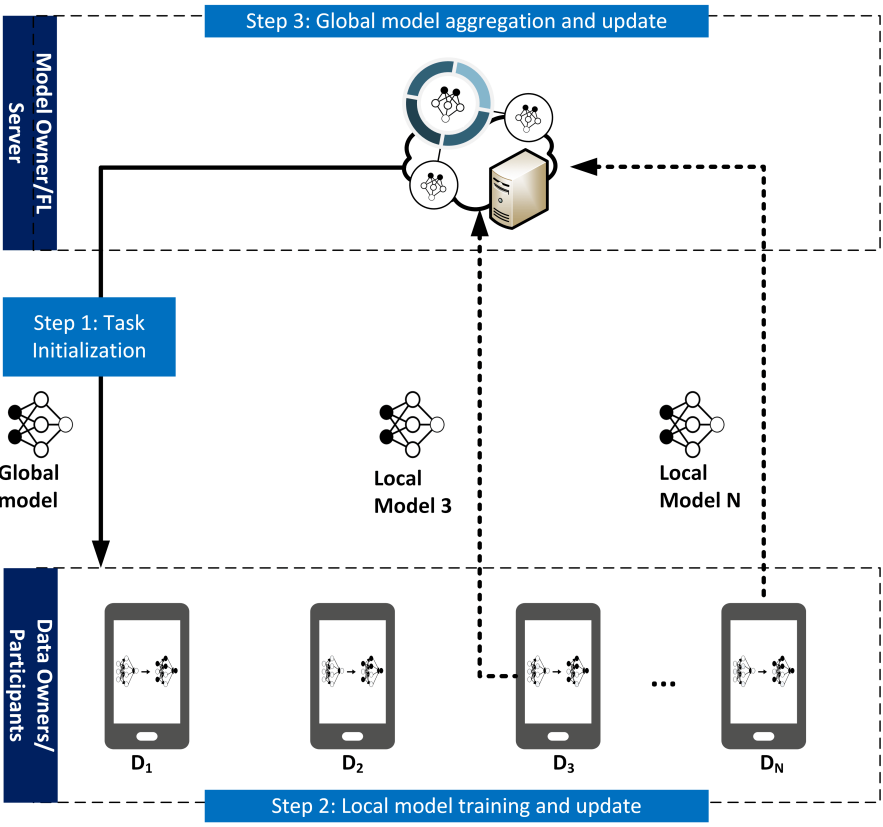
\includegraphics[width=0.6\textwidth]{Images/topologies/fl_topology.png}
        \decoRule
        \caption[FL topology]{Typical FL topology: \href{https://ieeexplore.ieee.org/document/9060868}{URL}.}
        \label{fig:FL topology}
\end{figure}

% operation/ basic loop
\subsection{Typical Federated Training Process}
FL training is a continuous process. Each iteration is referred as a global epoch and can be broken down into three main steps:

\subsubsection{Task Initialization}
Before any training can begin, the server has to complete a series of necessary tasks. It must first determine whether training should continue; if the target accuracy has been met or there are no available clients, there is no point to do. Furthermore, the server must specify any parameters or hyperparameters that are under its responsibility. FL design is flexible; factors such as learning rate may be controlled centrally by the server or by the clients.

After deciding how the training will proceed, the server must select \(N\) clients to participate. Clients may be chosen at random, based on eligibility requirements, etc. Finally, the server broadcasts the weights of the global model, together with any relevant metadata such as training parameters or a training program.

\subsubsection{Local Training} % A B
Upon receiving the global model, each selected client locally computes an update to it using their private data. This update is referred to as a local model. Training is carried out in accordance with any training parameters or programs that are provided. The objective \(f\) of a selected client \(n\) is to minimize its loss function \(L\) depending on the weights of the global model \(w_g\) and the local data \(d_i\):
\begin{equation}
    f_n \left( w_g \right) = \argmin_{n\in N} L\left( w_g ; d_n \right)
	\label{eqn:FL, Objective of a selected client}
\end{equation}

Subsequently, any required transformation may be applied to the local model. Such transformations include quantization and compression to reduce communication time, adding differential noise to increase privacy, and others. The finalized local model weights are sent to the server, together with any relevant statistics, and the client waits till it is selected once more.

\subsubsection{Model Aggregation} % A B
The server collects and aggregates the local models to generate a new global model. The aggregation is implementation dependent; it might simply be averaging the models, or it could be biased toward some based on their statistics, how many times they have participated, and so on. The global model can be evaluated using server-accessible public data. The objective of the server is to minimize the global loss function:
\begin{equation}
    F \left( w_g \right) = \frac{1}{N} \sum_{n=1}^N f_n \left( w_g \right)
	\label{eqn:FL, Objective of the server}
\end{equation}

This process is repeated until the global loss function converges, target accuracy has been achieved etc.

\subsection{Federated Learning Settings} % B
FL can be used in a broad array of applications with significantly diverse contexts and constraints \cite{survey_B, survey_D}. An example of FL across data centers could be hospitals that cooperatively train a cancer recognition model utilizing data from their patient diagnoses. Moreover, a real-world application of IoT FL is the training of a next-word prediction model for Google's Gboard \cite{GBoard_FL} utilizing users' personal text messages. Table \ref{table:FL scenarios} seeks to describe two generalized FL scenarios and compare them with data center Distributed Learning (DL).

\renewcommand{\arraystretch}{1.3}
\begin{table}[H]
    \center
    \small
    \hspace*{-9mm} \makebox[0pt]{
        \begin{tabular}
            {
                p{0.16\textwidth}
                p{0.32\textwidth}
                p{0.32\textwidth}
                p{0.32\textwidth}
            } 
            \hline
            & \multicolumn{1}{c}{Data center DL} & \multicolumn{1}{c}{Data center FL} & \multicolumn{1}{c}{IoT FL}\\
            \hline
            Setting & Training is distributed among nodes in a data center. A centralized dataset is used. & Organizations collaborate to train a model utilizing data in their data centers. & A large number of IoT devices are utilized to train model with their private data.\\
            
            Data \mbox{Distribution} & Data is balanced across nodes. Clients can access the whole dataset. & \multicolumn{2}{p{0.67\textwidth}}{Data is created locally and is kept decentralized. A client cannot access other clients' data. Generally, data is not independently or identically distributed.}\\
            
            Data \mbox{Partition} & Flexible, data can be repartitioned arbitrarily during training. & Fixed, partition axis can be by example or by feature. & Fixed partitioning by example.\\
            
            Orchestration & Centrally orchestrated. & \multicolumn{2}{p{0.67\textwidth}}{The training is organized by a central server, which has no access to the training data.}\\
            
            Topology & Fully connected nodes in a cluster. & \multicolumn{2}{>{\centering}p{0.67\textwidth}}{Typically hub-and-spoke.}\\
            
            Scale & Typically 1 to 1000 nodes. & From a couple to a few hundred data centers. & Massively parallel, up to millions of clients.\\
            
            Availability &\multicolumn{2}{>{\centering}p{0.67\textwidth}}{Almost always available.} & Only a fraction of the IoT devices is available at any single time.\\
            
            Client \mbox{Reliability }& \multicolumn{2}{>{\centering}p{0.67\textwidth}}{Few to no failures.} & Unreliable, a part of the participating clients is expected to disconnect due to power or network issues.\\
            
            Addressability & \multicolumn{2}{>{\centering}p{0.67\textwidth}}{Clients are identifiable and can be addressed explicitly.} & Generally unaddressable to enhance privacy.\\
            
            Client \mbox{Statefulness} & Statefull, nodes can participate in every epoch, carrying state from one to the next. & Any, design depended. & Mostly stateless, clients will most likely participate in only one epoch before being replaced.\\
            
            Primary \mbox{Bottleneck} & Computation. In a data center, a very fast network between nodes can be assumed. & Can be either computation or communication, problem depended. & Both, IoT tend to have low processing power and operate on slow connections (e.g. wifi).\\
        \end{tabular}
    }
    \caption{FL scenarios in comparison with data center distributed learning.}
    \label{table:FL scenarios}
\end{table}
\renewcommand{\arraystretch}{1}

% problems outlook
\subsection{Unique characteristics \& challenges of FL}
Aside from the standard challenges associated with ML development, there are a number of obstacles specific to FL. These issues distinguish the federated setting from more traditional problems such as private data analysis and data center DL. \cite{FL_comprehensive_survey, survey_B, survey_C, survey_D, survey_E}

\subsubsection{Expensive communication} % E
Communication is a critical bottleneck in many FL applications. In traditional data center DL, the communication environment is assumed to be perfect, with low latency, high bandwidth and negligible to no packet loss. This assumption is not appropriate to FL training, as clients are expected to be in different locations and with varying amounts of resources. This is especially true in edge FL, where the on-device datasets are small and connections are slow and unreliable, resulting to a high communication to computation ratio.

\subsubsection{Heterogeneous devices} % E
Client computational and communication capabilities can vary greatly in FL. They may differ in architecture (CPU, GPU, FPGA) and resources such as clock speed and RAM availability. Furthermore, they may be networked using different technologies (e.g., 4G, 5G, wifi) with varying reliability and bandwidth. Finally, some of them may be less eager to participate. All this leads to random and unpredictable client disconnections, as well as the appearance of "stragglers" \cite{stragglers}, clients who take substantially longer to provide their updates than the rest and impede the entire process.

\subsubsection{Statistical heterogeneity} % E
It is frequently assumed in distribution optimization problems that the data are independent and identically distributed (IID). This is commonly violated in the federated setting, adding complexity to problem modeling, analysis, and solution evaluation. Data generation and collection are frequently uneven between clients, and the server is unable to collect or check the quality and distribution of their data due to privacy issues.

\subsubsection{Privacy and Security concerns} % E
The primary concern of FL apps is to protect the privacy of participating customers. However, malicious participants or third parties may be able to infer sensitive information from shared parameters, defeating one of FL's key goals. Furthermore, its mostly assumed that all participants are well-intentioned, yet this is not always the case. Malicious clients may try to undermine the model's accuracy or install backdoors into it by utilizing poisonous datasets.
    
\begin{figure}[H]
    \centering
        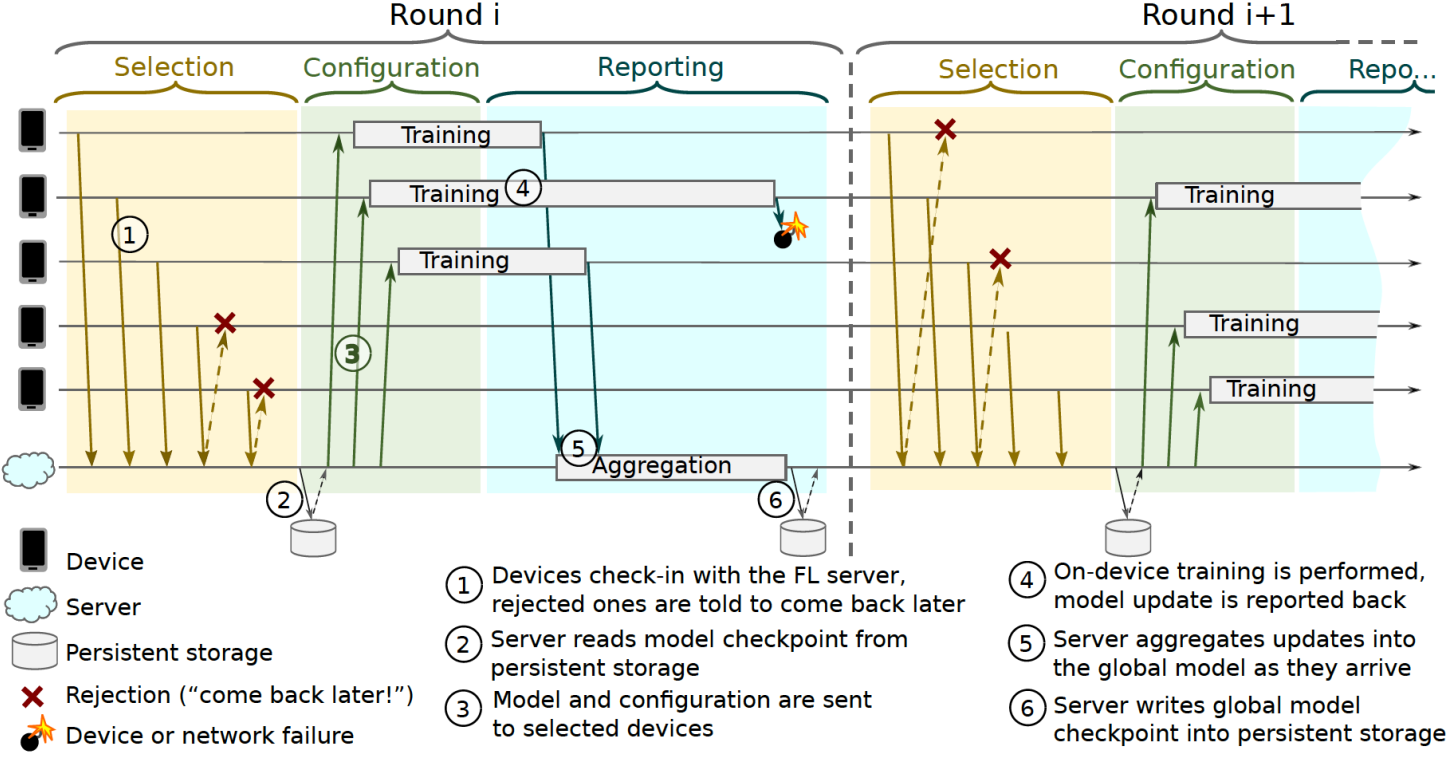
\includegraphics[width=1\textwidth]{Images/fl_protocol.png}
        \decoRule
        \caption[FL protocol]{FL protocol with stragglers, client disconnections and client selection: \href{https://ieeexplore.ieee.org/document/9060868}{URL}.}
        \label{fig:FL protocol}
\end{figure}

\subsection{Communication cost reduction}
To achieve a satisfactory model in FL, multiple rounds of training and communication between the server and the clients are required. Communication can be a big bottleneck if the ANN being trained is massive and has millions of parameters, or if the clients are under slow connections. As a result, a series of techniques for improving communication efficiency have been developed, which can be classified into three groups: increasing computation, decreasing communication size, and decreasing communication frequency.

\subsubsection{Edge and End Computation}
Increasing parallelism by selecting more clients each global epoch is an obvious technique to increase computation in edge devices. In general, client-wise parallelism is desirable, but it provides diminishing returns as the number of participating clients increases. Furthermore, if all of the connected clients are participating, this strategy is no longer applicable. Finally, there is the risk of rapidly exhausting the available datasets.

The most typical technique to increase computation is to have clients perform more local model updates per global epoch. This can be achieved in two ways, more local epochs, i.e. more passes through the local dataset, or smaller batch size, i.e. more updates per pass through the local dataset. In traditional DL, such techniques tends to produce negative effects like overfitting. On the other hand, FL algorithms, due to their model averaging, produce regularization effects equivalent to dropout, ultimately increasing the accuracy of the model under training.

While these techniques are effective, having too many local updates between communication rounds can have a negative impact. To begin with, local models may diverge too much from each other, especially when under non-IID data distribution, significantly decreasing the convergent rate of the global model. As a result, additional training is required, defeating the aim of these techniques.

Another concern is that the likelihood of stragglers occurring is considerably increased due to client heterogeneity. Clients with fewer resources will take disproportionately longer to complete the additional computations, widening the gap between them and the faster ones. Since simulations are most often used when developing FL algorithms, researchers frequently overlook this issue.

\subsubsection{Model Compression}
These techniques, which are extensively employed in DL, attempt to decrease the amount of the communicated updates. The weights of the model under training make up the majority of the updates; applying transformations like sparification, quantization, and subsambling to them can reduce the size of the updates. In general, they are classified into two types: structured updates, which attempt to select what information is sent, and sketched updates, which attempt to compress the communicated information.

Structured updates require that updates adhere to a set, reduced format. This is possible in multiple ways, like putting a predermined per-client mask on the model after training to sparsify it. Another method is to instruct a client to train and communicate only specific layers or pieces of them. A more complex alternative is for the server to apply dropout to the global model in order to create a submodel, which the clients train, and the server maps back to the global model during aggregation. In general, these methods try to shift the responsibility of compression to the server, with the aim to make it more predictable and correct its error.

Sketched updates refer to techniques that encode the update in one side and decode in the other. One such method is probabilistic quantization \cite{probabilistic_quantization}, in which the update matrices are vectorized and quantized for each scalar. Another option is to use a random mask like in a structure update, with the difference that it is randomly generated by the client and communicated to the server together with the encoded local model.

All these methods can be lossy and introduce error as a result of information loss. This error can be characterized as noise, which in most cases has a mean value of zero due to the nature of the compression algorithms commonly used. As such, the averaging of the FL algorithms can reduce it or even eliminate it from the accumulation of the local updates. For this to be true in practice, a large number of clients must be participating, which that is not always achievable. Moreover, as there is only one global model at any given time, any error in server-to-client communication cannot be reduced.

\subsubsection{Importance-based Updating}
By sending only what seems important, importance-based updating aims to reduce the volume of communication. Based on the observation that most parameters in an ANN are close to zero or hardly vary \cite{observation_parameters}, this can be done in a fine-grained manner by sending to the server only a small percentage of the model parameters. It can also be applied in a coarse-grained way by asking clients to review their updates and send them only if they think they would help the overall model. These techniques have demonstrated that, when applied properly, they can occasionally reduce communication while also increasing accuracy and convergence rate. In contrast, they may produce the opposite effects if used excessively.

\subsection{Systems heterogeneity}
The previously discussed systemic characteristics of FL aggravate issues like straggler mitigation and fault tolerance. The slowest participating client has a significant impact on the duration of a global epoch. They can substantially impede training speed, thus removing them from the process is generally considered. Furthermore, if the server waits indefinitely for the client updates and a client disconnects without notifying, the entire system would hang. These issues are especially prevalent in on-edge setting where there is little information or control over the clients' resources.

FL algorithms must be able to handle heterogeneous hardware and resist against random and unpredictable client drops. A frequent option is to disconnect clients who have not responded within a predetermined amount of time. Additionally, using more clients per epoch than necessary and accepting updates from those who respond first can help to eliminate stragglers. While effective, such strategies can induce biases in favour of the datasets of the fastest clients, reducing the overall accuracy of the model.

More sophisticated proposed solutions include intelligent client selection by only accepting clients that report their resources prior participating or tracking statistics on their overall performance. Such methods are not always feasible since they may jeopardize the privacy of the clients. A major portion of FL research employs simulations and avoid these problems, letting these challenges the least explored.

\subsection{Data distribution}
A dataset is independent and identically distributed (iid) if each example in it has the same probability distribution as the others and all are mutually independent. Models' accuracy, convergence rate, and fairness can all be degraded by training on non-iid datasets. Traditional ML avoids these issues by using a single, massive dataset that the designer is allowed to manipulate. On the other hand, FL encompasses a set of smaller datasets that could differ statistically from one another, and the designer may not be in control of or even aware of these differences. Ideally, a global dataset could be established by aggregating all of these small local datasets, however in reality this is impossible because the data cannot be centralized.

\begin{figure}[H]
    \centering
        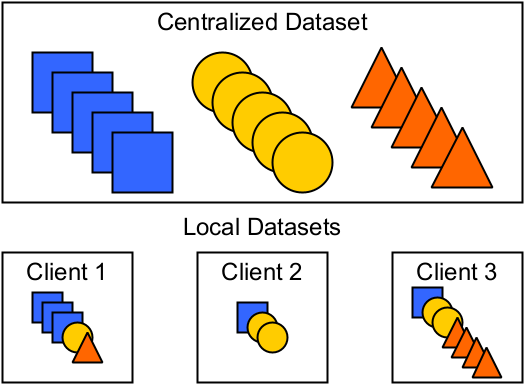
\includegraphics[width=0.6\textwidth]{Images/block_diagrams/data_distribution.png}
        \decoRule
        \caption[Data distribution]{Centralized Dataset vs. Local Datasets. When distributed unevenly among the clients, the same data can behave as non-iid.}
        \label{fig:Data distribution}
\end{figure}

\subsubsection{Non-identical client distributions}
A global dataset used during FL may not be iid for a variety of reasons. First of all, a client's private dataset may locally violate independence, but this can usually be fixed via local shuffling. The statistical variations between the local datasets are more significant.

The distribution of a local dataset \(P_i(x,y)\) can be rewritten as \(P_i(y|x)P(x)\) and \(P_i(x|y)P(y)\), where \(x\) and \(y\) are the input-output pairs. The distributions of at least two clients, I and j, must differ for the data to be non-iid, that is \(P_i \neq P_j\). There are several causes for this, including:

\begin{itemize}
  \item \emph{Feature distribution skew} (covariate shift), \(P_i(x) \neq P_j(x)\):\\
  Even if \(P_i(y|x) = P_j(y|x)\), the marginal distributions \(P(x)\) may differ. This is frequent in the domain of handwriting recognition, where two clients may write the same text in a different writing style.
  
  \item \emph{Label distribution skew} (prior probability shift), \(P_i(y) \neq P_j(y)\):\\
  Even if \(P_i(x|y) = P_j(x|y)\), the marginal distributions \(P(y)\) may differ. This is common when clients are bound to specific locations. Clients from different areas may use different terms and phrases depending on their local accent and lingo.
  
  \item \emph{Same label, different features (concept drift)}, \(P_i(x|y) \neq P_j(x|y)\):\\
  Even if \(P_i(y) = P_j(y)\), the marginal distributions \(P(x|y)\) may differ. The same label \(y\) can have different meaning for different users based on their culture and standard of leaving. Images of clothes, for example, can vary greatly according on location.
  
  \item \emph{Same features, different label (concept shift):}, \(P_i(y|x) \neq P_j(y|x)\):\\
  Even if \(P_i(x) = P_j(x)\), the marginal distributions \(P(y|x)\) may differ. This is very common with labels that reflect sentiment. As an example, clients living in cold climates may describe the same weather phenomena differently than clients lining in warm or temperate climates.
  
  \item \emph{Quantity skew}:\\
  Clients can generate and save different amounts of data. This is dependent on a variety of factors, including available data storage, local data retention laws, and the habits of their users.
  
  \item \emph{Violations of independence}:\\
  Throughout training, the distribution may change at any time. Clients may connect or disconnect, or their local datasets may be exhausted. Furthermore, if clients are available at specific times of day due to solstice, a strong regional bias is imposed. Finally, because the clients own their own datasets, they can modify them at any time during training.
  
  \item \emph{Dataset shift}:\\
  The FL participants might not be indicative of the end users. For instance, clients with inferior devices may be underrepresented as a result of any eligibility criteria used during client selection.
\end{itemize}

A real-world FL dataset may have any combination of these effects. Due to the difficulties of generating such datasets and examining algorithms built on them, most research tends to concentrate on one or two of them. Depending on the Fl scenario under training, different distribution skew effects may aplly and different mitigation strategies may be required.

\subsubsection{Dealing with non-iid distributions}
Existing algorithms can be modified, either by altering their parameters and hyperparameters or by sophisticating features like client selection. While adjusting other parameters, reducing batch size and increasing local epochs can be increase model accuracy, but excessive use may hurt convergence rate and lengthen training time. Metalearning approaches could be used to discover an ideal equilibrium.

It has been demonstrated that system heterogeneity and data heterogeneity interplay. By discarding straggles, unique and useful data could be wasted, degrading the model's fairness and accuracy. Stragglers can partially work, by personalizing parameters or reparameterizing on the fly, according to their resources. In this way, their local datasets can be exploited without slowing down the overall process.

Another approach is for the server to request data distribution statistics from the clients. With this information, the server can select those that will result in a balanced distribution. In addition, the server may be able to share some relevant publicly available data with the clients in order to rebalance their datasets. If no such data are available, willing clients may, if practical, provide their datasets to aid in the overall training process. These techniques can alleviate non-iid distribution problems, but they require additional communication and bandwidth. Additionally, they have the potential to compromise privacy, which would undermine one of FL's main goals.

Similarly, frameworks for multitask learning may be employed. Clients can train their local personalized models concurrently with the global model and share knowledge between them. Such techniques may not always be available as they demand greater processing and memory resources from the clients.

\subsection{Privacy and Security}
One of FL's key goals is to protect participants' privacy by simply requesting them to share model parameters and not any of their personal information. Additionally, FL wants to improve the model's fairness and accuracy by incorporating personal data. However, if any FL participant is malicious, these goals could be defeated. Model updates obtained from them can be used to reconstruct data, and poisoning attacks can corrupt the model.

\subsection{Types of Attacks} % D

\begin{itemize}
  \item Data poisoning attacks\\
  In order to lower the accuracy of the model and add biases, these attacks introduce tainted data that violate the dataset's integrity. Model skew attacks \cite{Model_skewing_attacks} and feedback weaponization\cite{feedback_weaponization} fall within this group. The goal of model skew attacks is to decrease the model's accuracy by obfuscating or distorting the boundaries between the classifiers. Feedback weaponization, on the other hand, tricks the model into misclassifying certain labels to introduce biases against them.
  
  \item Adversarial attacks \footnote{Also called model poisoning.}\\
  Adversarial attacks \cite{adversarial_attack} involve specially crafted data that have designed to be consistently misclassified by the model. They can be subdivided to non-targeted and targeted. Non-targeted attacks try to evade being correctly classification during inference, any incorrect result is acceptable. Targeted attacks aim to incorporate backdoors into the model, that means manipulate the network to give specific erroneous inference for certain inputs.
  
  \item Inferring Attacks\\
  Attacks of this kind aim to gain information about the participants and their data, and can be classified into two categories. The first one is tracing attacks, which aim to detect whether a client is actively participating into training. The second one reconstruction attacks, which aim to recreate examples used in training, or features of them.
  
  Such attack can perpetrated using model extraction algortihms and Generative Adversarial Networks \cite{GAN_attack} (GANs). GANs is a ML technique where two competing ANNs are trained, a generator network and a discriminator network. The generator tries to create fake data while the discriminator tries to discern real data from the fake by analyzing the output of the discriminator. After some training, the generator can create data that closely resembles the real ones using the statistics learned by the classifier.
  
  A GAN attack seeks to infer as much useful information as possible about elements in a target class that are not under its possession. The GAN tries to mimic samples of that class, mislabels them and feeds them to the ANN under federated training. The rest of the participants must then work harder to discriminate between the target class and the mislabeled class, resulting in additional knowledge about the target class in the global model. This process is repeated until convergence, and the GAN has enough information to reliably reconstruct samples from the target class that approximate the original examples. 
  
  This attack can be generalized to any number of classes and users, as well as any type of collaborative learning. If the server or another entity with access to the victim's communications is the malicious actor,it can be made more efficient by using the victim's local updates rather than the global model.
\end{itemize}

\begin{figure}[H]
    \centering
        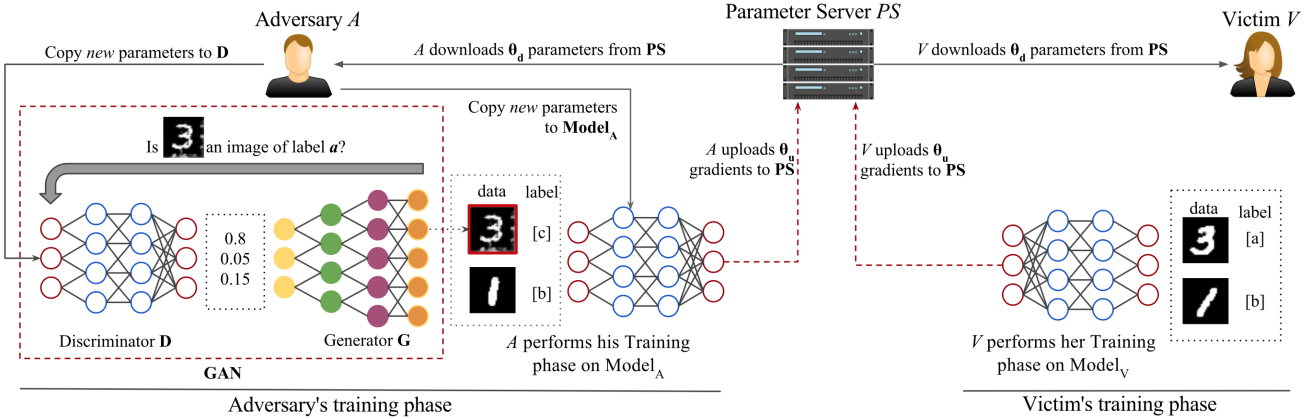
\includegraphics[width=1\textwidth]{Images/topologies/gan_fl.png}
        \decoRule
        \caption[GAN attack]{GAN attack. The adversary mimics images of class \emph{a}, labels them as class \emph{c} and uses them to train the collaborative model. To distinguish between these two classes, the model will require more information from the victim. The adversary does not need to have any true samples.: \href{https://arxiv.org/abs/1702.07464}{URL}.}
        \label{fig:GAN attack}
\end{figure}

\subsubsection{Countermeasures}
FL algorithms are somewhat resistant to the aforementioned attacks due to the regularization effect of averaging local models. Data poisoning and adversarial attacks require a sizable portion of the dataset to be tainted in order to succeed. Additionally, inferring attacks demand that the malicious actor go through numerous training epochs. In an IoT environment since most clients, if they are even chosen, will only participate once. Even when several malicious clients collude, the is a very small probability of achieving their goals.

Such scale is quite challenging to achieve in an environment closer to the datacenter, making it much more vulnerable. Furthermore, clients might seek stronger privacy guarantees as the server might not always trustworthy. For these reasons, further measures for protecting privacy and security are necessary.

An additional level of security can be provided with minimal adjustments to the FL protocol, by scanning the clients' updates for unusual patterns. Repeated updates with outlandish values could be a sign that a client is attempting to corrupt the model. Furthermore, the updates of clients that try to inject backdoors frequently resemble one another, which is rare, especially in a non-iid dataset. Such methods can improve the security of the model, but require plain-text access to the local updates, which is not always available due to privacy enhancements based on cryptography.

Clients might request further privacy protections, particularly if they don't trust the server or the connection between them. Secure Multi-Party Computation (MPC) \cite{MPC}, a subfield of cryptography, can be utilized to accomplish that. MPC simulate a trustworthy third party between two or more collaborating parties. Its homomorphic encryption techniques, which allow mathematical operations to be performed directly on cyphertexts and enable the server to aggregate the local models without having access to their plain-text contents, are particularly helpful. As a result, privacy can be ensured, albeit at a high computational cost that comes with cryptographic operations.

The state of the art method to enhance model security and restrict information exposure is differential privacy (DP) \cite{GAN_attack}. The fundamental tenet of DP is that by blurring a model's weights, they can not be associated with the data they were produced with. In FL, clients add random noise\footnote{Usually Gaussian.},with a mean value zero, to their local updates prior sharing them with the server. In addition of concealing the clients, this technique hinders dackdoor injections to the model, as the malicious clients need to send a precise set of parameters to achieve their goals.


\begin{figure}[H]
    \centering
        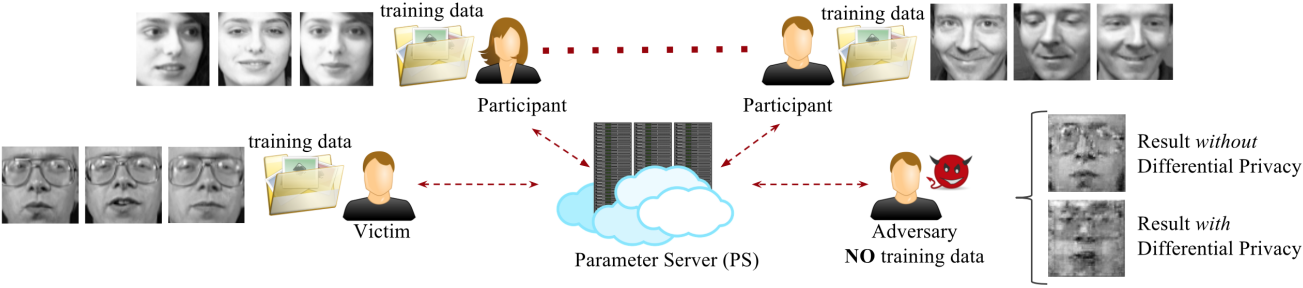
\includegraphics[width=1\textwidth]{Images/topologies/dp_on_gan_attack.png}
        \decoRule
        \caption[GAN attack under Differential Privacy]{Effect of Differential Privacy on a GAN attack.: \href{https://arxiv.org/abs/1702.07464}{URL}.}
        \label{fig:GAN attack under Differential Privacy}
\end{figure}

Theoretically, under DP transformation, the accuracy of the model and its convergence rate won't be impacted as the noise should vanish during aggregation. In practice, several samples are necessary to generate a distribution with a mean value close to zero, thus FL must be scaled appropriately. Finally, as attacks get more sophisticated, these countermeasures might not be effective and combinations of them or new ones are required.

%types
% \subsection{Categorization?} % C12:5 +B88
%     horizontal - vertical - transfer learning?
%     \subsubsection{Architectures for a federated learning system}
\chapter{Related Work}
\label{Chapter-Related-Work}

% Todo: Edit to your liking
\section{Training Datasets}
Common datasets and FL datasets from TF.
\section{FedAvg}
\section{CE-FedAvg}
\section{Evolution of FL}
Fig 5 from A review of applications in federated learning

\section{quantization?}

\section{The FPGA Perspective}
\section{Thesis Approach}

\chapter{Robustness Analysis}
\label{Chapter-Robustness-Analysis}

Maybe this need its own chapter\\
Developed FL architecture. Server - Client architecture, communication protocol, tf embeddment. Interface - code agnostic of NN design and training.

The experiments from the reviews. Add a prologue to show why they exist. Remake the supplementary ones with the latest settings.


% Todo: Edit to your liking
\section{Experiment A}
\section{Experiment B}

\chapter{FPGA Implementation}
\label{Chapter-FPGA-Implementation}

\section{Tools Used}
\subsection{Vivado IDE}
\subsection{Vivado High Level Synthesis (HLS)}
\subsection{Vivado SDK}

\section{FPGA Platforms}

\chapter{Results}
\label{Chapter-Results}

\section{Specification of Compared Platforms}
\section{Power Consumption}
\section{Energy Consumption}
\section{Throughput and Latency Speedup}
\section{Final Performance}

\chapter{Conclusions and Future Work}
\label{Chapter-Conclusions-and-Future-Work}

\section{Conclusions}
\section{Future Work}

\include{Chapters/08-test}

%----------------------------------------------------------------------------------------
%	THESIS CONTENT - APPENDICES
%----------------------------------------------------------------------------------------

\appendix % Cue to tell LaTeX that the following "chapters" are Appendices

% Include the appendices of the thesis as separate files from the Appendices folder
% Uncomment the lines as you write the Appendices

% \include{Appendices/AppendixA}

%----------------------------------------------------------------------------------------
%	BIBLIOGRAPHY
%----------------------------------------------------------------------------------------

\cleardoublepage
\phantomsection
\addcontentsline{toc}{chapter}{References}
\printbibliography

%----------------------------------------------------------------------------------------

\end{document}
